%\documentstyle[aas2pp4,epsf]{article}
%%%\documentstyle[aaspp4,epsf]{article}
%\documentstyle[12pt,aasms]{article}    % this is for a preprint
%(single-spaced)
%\documentstyle[aaspp4,epsf]{article} % this is for small print
%\documentstyle[12pt, aaspp4]{article}

%\documentstyle[11pt,aaspp]{article}
%\documentclass[12pt, preprint]{aastex} 

%\documentclass[manuscript]{aastex}
\documentclass[apj]{emulateapj}

%\documentclass[12pt, preprint,numberedappendix]{emulateapj}
%\documentstyle[12pt,aasms]{article}    % this is for submittal
                                       % (double-spaced)

%\documentstyle[12pt,aasms]{article}   \usepackage{emulateapj5} 

\usepackage{graphicx} 
\usepackage{graphics}                       
\usepackage{amsmath}
\usepackage{hyperref}
\usepackage{amsfonts}
\usepackage{amsmath}
\usepackage{amssymb}
\usepackage{amsthm}
\usepackage{subeqnarray}
%\bibliographystyle{apj}

\newcommand{\delad}{\nabla_{\rm ad}}
\newcommand{\delrad}{\nabla_{\rm rad}}
\newcommand{\emgr}[1]{\emph{ \color{gray} #1}}

\newcommand{\ie}{i.e.\ }
\newcommand{\eg}{e.g.\ }
\newcommand{\p}{\partial}
\newcommand{\xv}{\vc{x}}
\newcommand{\kv}{\vc{k}}
\newcommand{\brak}[1]{\langle #1\rangle}


\newcommand{\gcc}{\;\mathrm{g\; cm^{-3}}}
\newcommand{\gsc}{\;\mathrm{g\; cm^{-2}}}
\newcommand{\cm}{\; {\rm cm}}
\newcommand{\mm}{\; {\rm mm}}
%\newcommand{\ps}{\; {\rm s^{-1}}}
\newcommand{\km}{\; {\rm km}}
%\newcommand{\au}{\; \varpi_{\rm AU}}

\newcommand{\AU}{\; {\rm AU}}
\newcommand{\yr}{\; {\rm yr}}
\def\K{\; {\rm K}}

\newcommand{\vcs}[1]{\mbox{\boldmath{$\scriptstyle{#1}$}}}
\newcommand{\vc}[1]{\mbox{\boldmath{$#1$}}}
\newcommand{\nab}{\vc{\nabla}}
\DeclareMathSymbol{\varOmega}{\mathord}{letters}{"0A}
\DeclareMathSymbol{\varSigma}{\mathord}{letters}{"06}
\DeclareMathSymbol{\varPsi}{\mathord}{letters}{"09}

\newcommand{\Eq}[1]{equation\,(\ref{#1})}
\newcommand{\Eqs}[2]{equations (\ref{#1}) and~(\ref{#2})}
\newcommand{\Eqss}[2]{equations (\ref{#1})--(\ref{#2})}
\newcommand{\Eqsss}[3]{equations (\ref{#1}), (\ref{#2}) and~(\ref{#3})}
\newcommand{\App}[1]{Appendix~\ref{#1}}
\newcommand{\Sec}[1]{Sect.~\ref{#1}}
\newcommand{\Chap}[1]{Chapter~\ref{#1}}
\newcommand{\Fig}[1]{Fig.~\ref{#1}}
\newcommand{\Figs}[2]{Figs.~\ref{#1} and \ref{#2}}
\newcommand{\Figss}[2]{Figs.~\ref{#1}--\ref{#2}} 
\newcommand{\Tab}[1]{Table \ref{#1}}

\newenvironment{packed_item}{
\begin{itemize}
  \setlength{\itemsep}{1pt}
  \setlength{\parskip}{0pt}
  \setlength{\parsep}{0pt}
}{\end{itemize}}

%\newcommand{\delad}{\nabla_{\rm ad}}
%\newcommand{\delrad}{\nabla_{\rm rad}}
\newcommand{\Rg}{\mathcal{R}}
\newcommand{\RB}{R_{\rm B}}
\newcommand{\co}{_{\rm c}}
\newcommand{\di}{_{\rm d}}
\newcommand{\cb}{_{\rm RCB}}
\newcommand{\surf}{_M}
\newcommand{\mc}{m_{\rm c \oplus}}
\newcommand{\mcn}[1] { m_{ \rm c #1 \oplus} }
\newcommand{\MC}{M_{\rm crit}}
\newcommand{\au}{a_\oplus}
\newcommand{\aun}[1]{ a_{#1\oplus} }

\begin{document}
\bibliographystyle{apj}

\shortauthors{Piso \& Youdin}

\title{On the Minimum Core Mass for Giant Planet Formation}
\author{Ana-Maria A. Piso}
\affil{Harvard-Smithsonian Center for Astrophysics}
\author{Andrew N. Youdin}
\affil{JILA, University of Colorado at Boulder}

\begin{abstract}
The core accretion model proposes that giant planets form by the accretion of gas onto a solid protoplanetary core. Previous studies have found that there exists a ``critical core mass'' past which hydrostatic solutions can no longer be found and unstable atmosphere collapse occurs. This core mass is typically quoted to be around $10 M_{\oplus}$. In standard calculations of the critical core mass, planetesimal accretion deposits enough heat to alter the luminosity of the atmosphere, increasing the core mass required for the atmosphere to collapse. In this study we consider the extreme case in which planetesimal accretion is negligible and Kelvin-Helmholtz contraction dominates the luminosity evolution of the planet. We develop a two-layer atmosphere model with an inner convective region and an outer radiative zone that matches onto the protoplanetary disk, and we determine the minimum core mass for a giant planet to form within the typical disk life timescale for a variety of disk conditions, which we denote as  \textit{critical core mass}.  We find that the absolute minimum core mass required to nucleate atmosphere collapse within the disk lifetime is smaller for planets forming further away from their host stars. Moreover, the critical core mass is strongly dependent on disk temperature, opacity and mean molecular weight of the gas. Our results yield lower mass cores than corresponding studies for large planetesimal accretion rates. %We therefore show that it is easier to form a planet by growing the core first, then accreting a massive gaseous envelope, rather than forming the core and atmosphere simultaneously.

\end{abstract}

\section{Introduction}
\label{intro}

Current theories of giant planet formation postulate that these planets form either through core accretion (e.g., \citealt{harris78}, \citealt{mizuno78}, \citealt{stevenson82}, \citealt{boden86}, \citealt{wuchterl93}, \citealt{pollack96}, \citealt{dangelo11}), where solid planetesimals collide and grow into a massive solid core which then accretes a gaseous envelope, or due to a gravitational instability in the protoplanetary disk that leads to fragmentation of the disk into self-gravitating clumps (e.g., \citealt{harris78}, \citealt{boss97}, \citealt{rafikov05}, \citealt{kratter10}, \citealt{dangelo11}).  %quote murray-clay, kratter 10, rafikov 05, etc.

Standard core accretion models (e.g., \citealt{stevenson82}, \citealt{rafikov06}) assume that the core and the atmosphere grow simultaneously, and that planetesimal accretion deposits enough heat to alter the luminosity of the atmosphere, increasing the core mass required for the atmosphere to collapse. These studies consider that the planet atmosphere is in a steady state at all times, where all the incoming energy from planetesimal accretion is radiated away by the envelope. The core and the atmosphere grow simultaneously, and the mass of the envelope is a function of the core mass. As the atmosphere mass becomes comparable to the mass of the solid core, hydrostatic balance no longer holds and runaway gas accretion commences. For a set of disk conditions it is therefore found that there is one well-defined core mass past which hydrostatic solutions no longer exist and unstable atmosphere collapse occurs: this is defined as the ``critical core mass''.  Standard calculations find the critical core mass to be about $10 M_{\oplus}$ (e.g., \citealt{stevenson82}, \citealt{rafikov06}).

%Standard static calculations of giant planet formation that consider planetesimal accretion as the main source of luminosity (e.g., \citealt{mizuno78}, \citealt{stevenson82}, \citealt{rafikov06}) assume that the atmosphere is at all times in a steady state at which the luminosity due to planetesimal accretion is fully radiated away by the atmosphere.  Therefore, for a given set of disk conditions, there is a maximum mass the core can have before the onset of unstable accretion: this is defined as the critical core mass.

Forming giant planets at wide separations in the protoplanetary disk poses theoretical challenges. On the one hand, gravitational instability generates objects that are too massive to explain the current observed properties of exoplanets (e.g., \citealt{rafikov05}). On the other hand, planetesimal accretion is slow at large distances in the disk, and therefore large cores may not be able to form before the dissipation of the gas in the disk (e.g., \citealt{rafikov06}). It would therefore be easier if giant planets could form from smaller cores which need less time to grow. 

In this study, we show that giant planets can grow faster from small protoplanetary cores that are fully formed before significant gas accretion occurs. In this scenario, the planetesimal accretion rate is significantly slowed down during the gas contraction phase of the atmosphere. This reduction can arise, for example, due to dynamical clearing, or due to the core having formed in the inner parts of the disk and migrated outwards. In this situation, the atmosphere evolution is dominated by the contraction of the envelope rather than planetesimal accretion. The atmosphere is no longer in a steady state, but rather it accretes gas as it loses energy through radiation. 

In our model we therefore assume that the luminosity evolution of the atmosphere is dominated by gas contraction, while the planetesimal accretion rate is negligible. As a result, the protoplanetary core has a fixed mass. We consider that the atmosphere evolves in time through stages of quasi-static equilibrium. Once the mass of the gaseous envelope becomes comparable to the mass of the solid core, the self-gravity of the atmosphere can no longer balance the pressure gradient and unstable hydrodynamic collapse commences. The time required for the atmosphere to grow to this stage is the characteristic growth time of the atmosphere. For a set of fixed gas and disk conditions, there exists a minimum core mass for which the atmosphere can grow on the time scale described above within the life time of the protoplanetary disk, which we define as the \textit{critical core mass}. 

We build a two-layer atmosphere model, with a convective inner region and a radiative outer region that matches smoothly on to the protoplanetary disk, and develop a cooling model that evolves the atmosphere in time. We aim to find the critical core mass for a giant planet to form before disk dissipation.

This paper is organized as follows. In section \ref{sec2} we describe the assumptions of our atmosphere model, and derive the basic equations that govern the structure and evolution of the atmosphere. In section \ref{analytic}, we present a simplified analytic model that predicts the qualitative behavior of the numerical model. We describe our numerical results in section \ref{KH}, and determine the critical core mass for planet formation during the life time of the protoplanetary disk in section \ref{critical}.  We discuss some of the approximations of our model in section \ref{neglected} and summarize our findings in section \ref{conclusions}.

   %We assume that the luminosity is primarily generated in the convective zone of the atmosphere, 



%Giant planets play a fundamental role in shaping the orbital structure of planetary systems, and in affecting the delivery of volatiles to terrestrial planets in the 

\section{Atmosphere Models}
\label{sec2}

In this section we derive the structure and evolution of a planetary atmosphere embedded in a protoplanetary disk in the absence of planetesimal accretion. In section \ref{model} we describe the assumptions of our model. Section \ref{struct} presents the equations describing the structure of a static planetary atmosphere.  In section \ref{BCs} we discuss our boundary conditions and the properties of our assumed protoplanetary disk, and review relevant length scales.  In section \ref{cooling} we develop a model to estimate the rate at which the atmosphere cools. %Finally, we combine these calculations into a quasi-static model for atmospheric evolution in section \ref{twolayer}.

\subsection{Basic Model Assumptions}
\label{model}

We develop a two-layer atmosphere model with the following assumptions:

\begin{enumerate}
\item The planet consists of a solid core of fixed mass and a two-layer atmosphere composed of an inner convective zone and an outer radiative region that matches smoothly on to the protoplanetary disk. The two regions are separated by the Schwarzschild criterion for convective instability (see section \ref{struct}). We denote the surface between the two regions as the radiative-convective boundary (RCB), which is henceforth defined by a radius $r=R\cb$.
\item The luminosity evolution of the atmosphere is dominated by Kelvin-Helmholtz contraction, while planetesimal accretion is negligible. As such, the core no longer grows and has a fixed mass.
\item The luminosity is assumed to be constant throughout the outer radiative region. Since the structure of the convective zone is independent of its luminosity, we do not need to make additional assumptions about the luminosity in this region.
\item The envelope evolves through stages of quasi-static equilibrium.
\end{enumerate} 

We use assumptions for the atmosphere geometry and composition similar to those of previous studies (e.g., \citealt{ikoma00}, \citealt{pn05}), as follows:

\begin{enumerate}
\item The atmosphere is self-gravitating, spherically symmetric and in hydrostatic balance.
%\item The outer boundary of the envelope matches smoothly onto the surrounding nebula.
\item The atmosphere consists of a hydrogen-helium mixture, with hydrogen and helium mass fractions of 0.7 and 0.3, respectively.
\end{enumerate}

The time dependence of the atmosphere structure equations may be taken into account either explicitly or implicitly. Some previous studies of atmosphere accretion (e.g., \citealt{stevenson82}, \citealt{wuchterl93}, \citealt{rafikov06}) consider static envelopes, in which the luminosity is solely supplied by planetesimal accretion and fully radiated away by the atmosphere. In other studies, the time evolution is explicitly taken into account and full time dependent models are developed (e.g., \citealt{ikoma00}). We follow an intermediate approach and consider quasi-static evolution. Our model for the atmosphere growth time is described in section \ref{cooling}. 


%\subsection{Length Scales}
%\label{scales}




%Some previous studies of atmosphere accretion (e.g., \citealt{stevenson82}, \citealt{wuchterl93}, \citealt{rafikov06}) consider static envelopes, in which the luminosity is solely supplied by planetesimal accretion and fully radiated away by the atmosphere. In other studies, the time evolution is explicitly taken into account and full time dependent models are developed (e.g., \citealt{ikoma00}). We follow an intermediate approach and consider quasi static evolution. Our model for the atmosphere growth time is described in section \ref{...}. 





%For the atmosphere structure, we develop a two-layer atmosphere model with the following assumptions:
%
%\begin{enumerate}
%\item The planet consists of a solid core of fixed mass and a two-layer atmosphere composed of an inner convective zone and an outer radiative zone that matches smoothly on to the disk, as mentioned above. The two regions are separated by the Schwarzschild criterion for convective instability (e.g., \citealt{thompson06}) 
%\item The luminosity evolution of the atmosphere is dominated by Kelvin-Helmholtz contraction rather than planetesimal accretion. 
%\item The luminosity is assumed to be constant throughout the outer radiative region.
%\item The envelope evolves through stages of quasi-static equilibrium.
%\end{enumerate} 

\subsection{Structure Equations and Boundary Conditions}
\label{struct}

An atmosphere in hydrostatic equilibrium is fully described by the following structure equations:

\begin{subeqnarray}
\label{eq:struct}
\frac{d P}{d r}&=&-\frac{G m}{r^2}\rho \slabel{eq:structa} \\
\frac{d m}{d r}&=&4 \pi r^2 \rho\slabel{eq:structb} \\
\frac{d T}{d r}&=&\nabla \frac{T}{P}\frac{d P}{d r}\slabel{eq:structc} \\
\frac{d L}{d r}&=&4 \pi r^2 \rho (\epsilon + \epsilon_g)\slabel{eq:structd}, 
\end{subeqnarray}

\noindent where $r$ is the radial coordinate, $P$, $T$ and $\rho$ are the gas pressure, temperature and density, respectively, $m$ is the mass enclosed by the radius $r$, $L$ is the luminosity from the surface of radius $r$, $\epsilon$ is the rate at which heat is generated due to internal sources, and $\epsilon_g \equiv -T \frac{ds}{dt}$ represents the heating per unit mass due to gravitational contraction, with $s$ the specific gas entropy. In our study we assume that there are no internal heat sources, and therefore $\epsilon=0$. The temperature gradient $\nabla \equiv \frac{d \ln T}{d \ln P}$ has different expressions depending on the primary means of energy transport throughout the atmosphere. We assume that energy can be transported either through radiation or convection. When the luminosity is carried by radiative diffusion, the temperature gradient is given by

\begin{equation}
\label{eq:delrad}
\nabla = \delrad \equiv \frac{3 \kappa P}{64 \pi G m \sigma T^4} L,
\end{equation}

\noindent where $\sigma$ is the Stefan-Boltzmann constant and $\kappa$ is the opacity. Equation (\ref{eq:delrad}) is valid when the atmosphere is optically thick, which is true throughout the entire atmosphere for our choice of opacity. Alternatively, when energy is transported outwards through convective motions, the temperature gradient becomes


\begin{equation}
\label{eq:delad}
\nabla = \delad \equiv \Big(\frac{d \ln T}{d \ln P}\Big)_{\mathrm{ad}},
\end{equation}
\\

\noindent where $\delad$ is the adiabatic temperature gradient. For an ideal gas of adiabatic index $\gamma$, $\delad=\frac{\gamma-1}{\gamma}$. The process that dominates energy transport throughout the atmosphere is determined by the Schwarzschild criterion (e.g., \citealt{thompson06}): the atmosphere is stable against convection when

\begin{equation}
\label{eq:schwarz}
\nabla < \delad
\end{equation}

\noindent and convectively unstable when the reverse is true. In order for convection to be effective, $\nabla \approx \delad$. Therefore, we find that the temperature gradient is given by $\nabla=\mathrm{min}(\delad, \delrad)$. 

In order for the equation set (\ref{eq:struct}) to be solvable, it has to be supplemented by an equation of state (EOS) that relates pressure, temperature and density $P=P(\rho, T)$, and an opacity law for $\kappa$. In our study, we assume an ideal gas polytropic EOS 

\begin{equation}
\label{eq:polyEOS}
P=K \rho^{\gamma}=K \rho^{1/(1-\delad)},
\end{equation}

\noindent with $K$ the adiabatic constant, determined by $\delad$. The adiabatic gradient is $\delad=2/5$ for a monatomic gas and $\delad=2/7$ for a diatomic gas. Additionally, the ideal gas law relates the pressure, temperature and density through

\begin{equation}
\label{eq:idealgas}
P=\rho \mathcal{R} T,
\end{equation}

\noindent with  $\mathcal{R}$ the reduced gas constant: $\mathcal{R}=k_b/(\mu m_p)$, $k_b$ the Boltzmann constant and $m_p$ the proton mass. The gas constant $\mathcal{R}$ depends on the mean molecular weight of the gas $\mu$, which is determined by the relative abundance of hydrogen and helium in the atmosphere. In this study we assume that the helium fraction only affects the molecular weight of the gas, and not the adiabatic index.% We show in section \ref{critcore} that this assumption does not affect the qualitative behavior of our solutions.

We assume an opacity power law of the form

\begin{equation}
\label{eq:opacitylaw}
\kappa=\kappa_0 \Big(\frac{P}{P_{\rm{ref}}}\Big)^{\alpha} \Big(\frac{T}{T_{\rm{ref}}}\Big)^{\beta},
\end{equation}  

\noindent with $\alpha$ and $\beta$ constants, $\kappa_0=2 F_{\kappa}$, and $T_{\rm{ref}}$ and $P_{\rm{ref}}$ reference temperature and pressure, respectively. To estimate $\alpha$ and $\beta$ we use the \citet{bell94} opacity laws for ice grains: $\alpha =0 $, $\beta=2$, $T_{\rm{ref}}=100$ K, and $F_{\kappa}=1$ (i.e., $\kappa_0=2$). We note that these values are valid only for low disk temperatures: $T_d \lesssim 100 K$. As such, we only consider cool atmospheres that form in the outer part of the protoplanetary disk ($a \geq 5$ AU).

\subsection{Boundary Conditions}
\label{BCs}


In what follows we first define several characteristic length scales that are important for this problem. \\

\textbf{The Core Radius} represents the physical radius of the protoplanetary core:

\begin{equation}
\label{eq:rc}
R\co \equiv \Big(\frac{3 M\co}{4 \pi \rho\co}\Big)^{1/3},
\end{equation}

\noindent with $M\co$ and $\rho\co$ the core mass and density, respectively. Since we assume that the core mass does not change with time, the core radius is also fixed for a given model. \\

\textbf{The Bondi Radius} represents the distance from the planet at which the thermal energy of the nebular gas is of the order of the gravitational energy binding the gas to the planet. It is defined as

\begin{equation}
\label{eq:RB}
R_{\rm B} \equiv \frac{G M_{\rm p}}{c_s^2}=\frac{G M_{\rm p}}{\mathcal{R} T\di},
\end{equation}

\noindent where $G$ is the gravitational constant, $M_{\rm p}$ is the total mass of the planet, $c_{\rm s}$ is the isothermal sound speed, defined as $c_{\rm s}=\Big(\frac{k_b T\di}{\mu m_p}\Big)^{1/2}$, and $\mathcal{R}$ is the reduced gas constant defined in section \ref{struct}.\\


\textbf{The Hill Radius} represents the distance at which the gravitational attraction of the planet and the tidal acceleration from the host star are the same. It is given by

\begin{equation}
\label{eq:RHill}
R_{\rm H} \equiv a \Big(\frac{M_{\rm p}}{3 M_{\odot}}\Big)^{1/3}.
\end{equation}

\noindent Outside the Hill radius, the gravity of the planet is too weak to affect the nebular gas. Consequently, the planet can only accrete gas that lies within its Hill sphere. \\

\textbf{The Disk Scale Height} is defined by

\begin{equation}
\label{eq:H}
H \equiv \frac{c_{\rm s}}{\Omega},
\end{equation}

\noindent where $\Omega$ is the Keplerian angular velocity. The disk scale height is a measure of the thickness of the protoplanetary disk. %Using equation (\ref{eq:diska}), we find that the scale height for our assumed disk model can be expressed as

%\begin{equation}
%\label{eq:H2}
%H=0.022 \sqrt{F_T} a^{9/7} \,\, \mathrm{AU}
%\end{equation}

For small planet masses, $R_{\rm B}<R_{\rm H}<H$. As the atmosphere becomes more massive, tidal truncation becomes more important than thermal constraints, and $R_{\rm H}<R_{\rm B}<H$. Finally, for high mass atmospheres the disk scale height becomes smaller than the Hill radius of the planet, and spherical symmetry breaks, as the planet is now affected by the vertical profile of the disk. In our study, we only accept atmosphere solutions that are spherically symmetric.

We assume a solid core of fixed mass $M\co$ with a radius given by equation (\ref{eq:rc}). We choose $\rho\co=3.2$ g cm$^{-3}$ (e.g., \citealt{pap99}). Furthermore, we assume the atmosphere extends out to the boundary of the Hill sphere, defined by equation (\ref{eq:RHill}). If the Bondi radius (defined in equation \ref{eq:RB}) is within the Hill radius, perturbations of the nebular gas still occur past the Bondi radius due to the gravitational influence of the planet. If, on the other hand, $R_{\rm B}>R_{\rm H}$, then the Hill radius is the more relevant truncation radius since material cannot be gravitationally bound to the protoplanet outside the Hill sphere. As such, it is always safe to choose the Hill radius as the outer boundary. We note, however, that we define the planet mass as only the mass enclosed within the Bondi radius if $R_{\rm B}<R_{\rm H}$.%, i.e. $M_{\rm{tot}}=M\co+M_{\rm{atm}}=M(<\text{min}(R_{\rm B}, R_{\rm H}))$.

The atmosphere matches smoothly onto the disk at the outer boundary. The temperature and pressure at the Hill radius have to therefore be given by the nebular temperature and pressure: $T(R_{\rm H})=T\di$ and $P(R_{\rm H})=P\di$. As a fiducial disk model, we use the minimum mass, passively irradiated model of  \citet{chiang10}. In this model, the surface density and mid-plane temperature are given by 

\begin{subeqnarray}
\label{eq:diskparam}
\Sigma\di&=&2200 F_{\Sigma} (a/\text{AU})^{-3/2}\,\, \text{g cm}^{-2} \slabel{eq:diska}\\
T\di &=& 120 F_T (a/\text{AU})^{-3/7} \,\,K, \slabel{eq:diskb}
\end{subeqnarray}

\noindent with $a$ the semi-major axis, and $F_{\Sigma}$ and $F_T$ normalization factors that adjust the disk mass and temperature relative to the minimum mass solar nebula (MMSN). In this study, we assume $F_{\Sigma}=F_T=1$. The resulting mid-plane pressure and disk scale height are given by 

\begin{equation}
\label{eq:Pd}
P\di=110  F_{\Sigma} \sqrt{F_T m_*} (a/\text{AU})^{-45/14} \,\, \text{dyn cm}^{-2}
\end{equation}
and
\begin{equation}
H=0.022 \sqrt{F_T} (a/\text{AU})^{9/7}\,\, \text{AU},
\end{equation}

\noindent respectively, for a molecular weight $\mu=2.35$. Here $m_* \equiv M_*/M_{\odot}$, where $M_*$ is the mass of the central star and $M_{\odot}$ is the mass of the Sun. We take $m_*=1$. 

%\subsection{Standards Methods of Solution}

%Analogously to the stellar evolution case, simply integrating the structure equations (\ref{eq:struct}) from one boundary to the other is not possible, since the boundary conditions are given both at the center and at the surface. In this case, the standard procedures for numerical integration are the shooting method or the Henyey method (\citealt{kippenhahn90}). The shooting method solves the boundary value problem by reducing it to an initial value problem: trial values are chosen for the parameters at one of the boundaries, then the equations are integrated and the resulting values at the other boundary are compared to the actual boundary conditions. The procedure is repeated until convergence is achieved. Alternatively, inward and outward integrations are carried to an intermediate fitting point, where they are fitted smoothly to each other. In the Henyey method, a trial solution for the whole interval is initially guessed, then gradually adjusted through subsequent iterations until the desired level of accuracy is achieved. In this study we use the shooting method --- we integrate inwards from the disk, and match at the core. The detailed numerical procedure is described in section \ref{twolayer}. 



\subsection{Virial Equilibrium and Global Cooling Model}
\label{cooling}

Section \ref{struct} provides the structure model for a static atmosphere. We now derive the time evolution of the atmosphere due to Kelvin-Helmholtz contraction between subsequent static models. 

We first describe the general ways in which planetary Klevin-Helmholtz contraction differs from the stellar case. An isolated sphere, such as a star, satisfies a simple global energy equation:

\begin{equation}
\label{eq:coolingstar}
L=\Gamma - \dot{E},
\end{equation}

\noindent where the total luminosity $L$ is balanced by the rate of heat generation $\Gamma$ (due to nuclear fusion in the case of a star) and the rate of change of the total energy of the sphere $\dot{E}$. The total energy of the sphere $E$ is given by the sum of the gravitational and internal energies: $E=E_{\rm G}+U$, with 

\begin{equation}
\label{eq:Eg}
E_{\rm G}=-\int_{M\co}^M \frac{G m}{r} dm,
\end{equation}
and
\begin{equation}
\label{eq:U}
U=\int_{M\co}^M u\, dm,
\end{equation}
where $u$ is the internal energy per mass.

A protoplanetary atmosphere that is not isolated, but rather embedded in a gas disk, satisfies a more complex cooling equation:

\begin{equation}
\label{eq:coolingglobal}
L=L\co+\Gamma-\dot{E}+e_{\mathrm{acc}}\dot{M}-P_M \frac{\partial V_M}{\partial t}
\end{equation}

This cooling model applies at any radius $R$ where the mass enclosed is $M$, for example the Bondi radius or the Hill radius. The $L$, $\Gamma$ and $\dot{E}$ terms are the same as in equation (\ref{eq:coolingstar}), and include the atmosphere from the core to the top boundary. In what follows we explain the additional terms in the cooling equation (\ref{eq:coolingglobal}). The first term $L\co$ is the luminosity from the solid core, and may include planetesimal accretion and radioactive decay. Since planetesimal accretion is negligible in our model, we set $L\co=0$. The fourth term on the right-hand side of equation (\ref{eq:coolingglobal}) accounts for the fact that gas is being brought in from a finite radius $R$ with a specific accretion energy $e_{\mathrm{acc}}$ given by $e_{\mathrm{acc}}=u-G M/R$. The last term represents the work done on a mass element as the atmosphere contracts. In the partial derivative the enclosed mass variable $m$ is kept fixed, and the derivative is evaluated at the surface with total enclosed mass $M$. We can think of this as rewriting the atmosphere structure equations (\ref{eq:struct}) in terms of $m$ rather than $r$, and taking into account that the thermodynamic quantities now also depend on the time $t$ (whereas time dependence is neglected in our static profiles). As such, $\partial / \partial t$ is the partial time derivative taken at constant mass. 

 %As we now take into account the time-dependence of the structure equations (\ref{eq:struct}),  In the 

 %In the cooling model given by equation (\ref{eq:coolingglobal}), the enclosed mass variable $m$ is kept fixed.  and take into account the time-dependence of the thermodynamic variables, which we neglected when obtaining static atmosphere models from equation (\ref{eq:struct}). This is equivalent to rewriting equation set (\ref{eq:struct}) with $m$ as the variable of integration; the partial 

%In the partial derivative we are keeping fixed the enclosed mass variable $m$ and we evaluate this term at the surface with total enclosed mass $M$. This is equivalent to rewriting the structure equations (\ref{eq:struct}) with $m$ as the variable of integration, and taking into account the time dependence of the thermodynamic variables explicitly.   The partial derivative $\partial / \partial t$ is therefore taken at fixed mass. 

%The partial derivative accounts for the fact that we are calculating this term at a fixed atmosphere mass, rather than total envelope mass that includes the mass accreted through the upper boundary. 

The global cooling equation (\ref{eq:coolingglobal}) can be derived from the local cooling equation (\ref{eq:structd}) and the virial theorem, which relates the internal and gravitational energy of the planet as follows:
\begin{equation}
\label{eq:virial}
E_G=-3 \int_{M_c}^M \frac{P}{\rho} dm + 4 \pi (R^3 P_M-R\co^3 P\co),
\end{equation}
where $P_M$ is the pressure at radius $R$ where the mass enclosed is $M$ and $P\co$ is the pressure at the core. The virial theorem is derived from the structure equations (\ref{eq:struct}). We defer the explicit derivation of equation (\ref{eq:coolingglobal}) to \App{sec:virial}.

%The global cooling equation (\ref{eq:coolingglobal}) can be derived starting from the local cooling balance. 



%Moreover, a self-gravitating protoplanetary atmosphere has to satisfy virial equilibrium. The virial theorem is derived by integrating the equation of hydrostatic balance (\ref{eq:structa}) and has the form

%\begin{equation}
%\label{eq:virial}
%E_G=-3 \int_{M_c}^M \frac{P}{\rho} dm + 4 \pi (R^3 P_M-R_c^3 Pc)
%\end{equation}
%
%Similarly to the cooling equation, it applies at any radius $R$ where the total mass enclosed is $M$. For an ideal gas of adiabatic index $\gamma$, equation (\ref{eq:virial}) leads to the following expression for the total energy:
%
%\begin{subeqnarray}
%E&=&(1-\xi)U+4 \pi (R^3 P_M-R_c^3 Pc) \slabel{eq:vira} \\
%&=&\frac{\xi-1}{\xi}E_G+\frac{4 \pi}{\xi} (R^3 P_M-R_c^3 Pc) \slabel{eq:virb}
%\end{subeqnarray}
%
%The global cooling equation (\ref{eq:coolingglobal}) can therefore be derived using equations(\ref{eq:coolinglocal}) and (\ref{eq:virial}). A detailed derivation is deferred to  \App{sec:virial}.




\section{Analytic Cooling Model}
\label{analytic}

In this section we derive a simplified analytic model for the atmosphere structure and evolution, based on the assumptions and equations described in section \ref{sec2}. We use this model to predict the qualitative behavior of our more detailed numerical model. %, and to explain expected scalings (\textbf{Maybe take out this sentence.})

We consider a two-layer atmosphere structure model as presented in section \ref{model}, and we make two key assumptions: we neglect the self-gravity of the atmosphere, and we assume that the outer radiative region is very thick and hence the pressure at the radiative-convective boundary is much larger than the disk pressure $P\di$. We will show in section \ref{KH} that these assumptions limit the applicability of this simplified model during the late and early stages of the atmosphere evolution, respectively. We also approximate the structure of the radiative zone as nearly isothermal, and note that this assumption is consistent with the numerical solutions (see section \ref{profiles}). 

As self-gravity is quantitatively important, we expect our analytic model to only provide scalings for the full numerical model rather than absolute values.


%We approximate the outer radiative zone of the atmosphere as nearly isothermal. Moreover, we do not take into account the self-gravity of the atmosphere in either region. We derive the structure of an isothermal non self-gravitating atmosphere is section \ref{iso}. 

We use the quasi-static model of section \ref{sec2} to derive expressions for the mass, energy and luminosity of a static non self-gravitating atmosphere. We use this to derive the time evolution of the atmosphere and determine the minimum core mass for runaway gas accretion in section \ref{coolingan}. We defer the details of our calculations to \App{sec:analytic}.


%In the next subsections we derive the structure and cooling behavior of a two-layer non self-gravitating atmosphere, deferring some of the calculations to \App{sec:analytic}. We estimate the temperature and pressure corrections at the radiative-convective boundary due to the fact that the outer radiative region of the atmosphere is not purely isothermal in section \ref{RCBcorr}. Finally, we derive the time evolution of the atmosphere and determine the minimum core mass for runaway gas accretion in section \ref{coolingan}.

%\subsection{Simplified cooling model}
%\label{coolingan}

%In this section we

%We now use a simplified version of the cooling model introduced in section \ref{cooling} in order to obtain an analytic cooling model. As before, we assume a polytropic equation of state and neglect self-gravity.

\subsection{Mass, Energy and Luminosity}
\label{MELan}

In this section, we derive simplified analytic expressions for the mass, energy and luminosity of the atmosphere.

Our assumption of a nearly isothermal radiative region yields simple expressions for the temperature and pressure at the radiative-convective boundary as a function of the nebular temperature and pressure. These expressions will helps us estimate the mass and energy of the atmosphere. We account for the departure from a perfectly isothermal layer (i.e., constant temperature and exponential pressure profile, see also equation \ref{eq:rhoiso}) by introducing two correction terms $\chi$ and $\theta$ such that

\begin{equation}
\label{eq:Tcb}
T\cb = \chi T\di
\end{equation} 
and
 \begin{equation}\label{eq:PcbRcb}
P\cb = \theta P_{\rm d} e^{R_{\rm B}/R\cb} \, ,
\end{equation}
where $\chi$ can be approximated as
\begin{equation}
\label{eq:chi}
\chi \simeq \Big(1-\frac{\delad}{\nabla_{\infty}} \Big)^{-\frac{1}{4-\beta}} ,
\end{equation}
with $\nabla_{\infty}=(1+\alpha)/(4-\beta)$ the radiative temperature gradient as $T, P \rightarrow \infty$. A simple analytic expression for $\theta$ is not possible. Both $\chi$ and $\theta$ depend on $\alpha$, $\beta$ and the adiabatic gradient $\delad$. For $\alpha=0$, $\beta=2$ and $\delad=2/7$, we find $\chi \approx 1.5$ and $\theta \approx 0.556$. Values for $\theta$ and $\chi$ for other choices of $\beta$ are summarized in \App{sec:analytic}, Table I. 

We then determine the density profile in the convective region of the atmosphere to estimate the mass of the atmosphere. Integrating the equation of hydrostatic balance (\ref{eq:structa}) and holding the mass fixed at $M\co$, we find

\begin{equation}\label{eq:rhoconv} 
\rho = \rho\cb \left[ 1 + {R_B' \over r} - {R_B' \over R\cb}  \right]^{1/(\gamma -1)},
\end{equation} 
where we define an effective Bondi radius,
\begin{equation}
R_B' \equiv {G M\co \over C_{\rm P} T\cb} = {\delad \over \chi} R_B
\end{equation} 
to simplify expressions, with $C_{\rm P}$ the specific heat at constant pressure.

From this we can calculate the mass of the convective region as

\begin{eqnarray} 
\label{eq:Matman}
M_{\rm atm} &=& 4 \pi \int_{R\co}^{R\cb} \rho r^2 dr \\
&\approx& {5 \pi^2 \over 4} \rho\cb {R_B'}^{5/2} \sqrt{R\cb}, % \approx 0.54 \rho\cb {R_B'}^{5/2} \sqrt{r\cb} \\
%&=& 0.54{R_B'^{3} \sqrt{\chi} \over  \sqrt{ \ln[P\cb/(\theta P\di)]}} \, .
\end{eqnarray}
in the limit $R\co \ll R\cb \ll R_B'$ and where $\gamma=7/5$ in the final expression. The mass in the isothermal region can be estimated as $M_{\rm iso} \sim 4 \pi \rho\cb r\cb^4/R_{\rm B}$ (see \App{sec:analytic} for a derivation).  We see that $M_{\rm{iso}} \ll M_{\rm{atm}}$ and therefore it can be neglected.


The total (thermal and gravitational) energy in an adiabatic atmosphere can be evaluated from the virial theorem (see section \ref{cooling}).  More simply, we use the result for temperature profiles in deep, but non-self-gravitating, convective regions:
\begin{equation}
T \approx {G M\co \over C_P r} = T\cb {R_B' \over r}\, .
\end{equation} 
The internal energy per unit mass of an ideal gas is thus $u = C_V T = (1 - \delad) G M\co/r$ and the specific energy  deep in the atmosphere is
\begin{equation}
e = e_g + u = -\delad {GM\co \over r} \, .
\end{equation} 
The total energy follows as
\begin{eqnarray} 
E &=& - 4 \pi \nabla_{\rm ad} G M\co \int_{R\co}^{r\cb} \rho r dr \\
&\approx& - 4 \pi P\cb {R_B'}^{1 \over \nabla_{\rm ad}} \left(\gamma-1 \over 3 - 2 \gamma\right)  R\co^{2\gamma-3\over \gamma-1}  \slabel{eq:Ean} \\ 
&\approx& - 8 \pi P\cb {R_B'^{7/2} \over \sqrt{R\co}}
%&\approx& -0.31 P\cb {(R_B / \chi)^{7/2} \over \sqrt{R\co}}
%&\approx& -0.31 P\cb {R_B'^{7/2} \over \sqrt{R\co}}
\end{eqnarray} 
when $\gamma = 7/5$. % and then revert to the standard Bondi radius $R_B = G M\co/(\Rg T\di)$ in terms of the disk temperature.

We note that the approximation in the energy expression of equation (\ref{eq:Ean}) is valid only deep in the adiabatic atmosphere, where  $\rho \propto r^{-1/(\gamma -1)}$ from equation (\ref{eq:rhoconv}).  As the energy scales as $\rho r^2 \propto r^{(2\gamma -3)/(\gamma - 1)}$, only polytropes with $\gamma < 3/2$ (i.e. $\gamma = 7/5$, but not $\gamma = 5/3$) have the bulk of energy at the bottom of the atmospheres.  Equation (\ref{eq:Ean}) is therefore only valid when $\gamma<3/2$. % We will thus focus on the $\gamma = 7/5$ case, even though dissociation occurs deep in real protoplanetary atmospheres.

Finally, we can estimate the luminosity that emerges at the radiative-convective boundary from equation (\ref{eq:structc}) assuming $\delrad=\delad$ at the radiative-convective boundary, as

\begin{equation} \label{eq:Lcb}
L\cb = {64 \pi G M\cb \sigma T\cb^4 \over 3 \kappa P\cb } \nabla_{\rm ad} \approx L\di {P_{\rm d} \over P\cb}, % \left({P\di \over P\cb}\right)%^{1+\alpha}
\end{equation} 
where we drop the pressure dependence from the opacity law (\ref{eq:opacitylaw}) and define 
\begin{equation} 
L\di \equiv {64 \pi G M\cb \sigma T_{\rm d}^4 \over 3 \kappa(T_{\rm d}) P_{\rm d}} \nabla_{\rm ad}\chi^{4-\beta}, 
\end{equation} 

 For $\beta = 2$ and $F_\kappa = 1$ in the opacity law (\ref{eq:opacitylaw}), this gives the \citet{bell94} opacity for icy grains.  By varying $F_\kappa$, dust depletion or enhancement can be considered.  Grain properties affect both $F_\kappa$ and $\beta$, which generally satisfies  $1/2 \lesssim \beta \lesssim 2$ (aside from discontinuities across sublimation regions, see \citealt{semenov03}).






%  The physical origin of this logarithm is the exponential increase of pressure with depth in the radiative zone.

\subsection{Simplified Cooling Model}
\label{coolingan}

We use the equations obtained in section \ref{MELan} to estimate the atmosphere mass $M_{\rm{atm}}$ for which $M_{\rm{atm}} \sim M\co$ and runaway accretion commences. We then use a simplified version of the cooling model developed in section \ref{cooling} to estimate the time elapsed until collapse. 

We can eliminate $R\cb$ from equation (\ref{eq:Matman}) using \Eq{eq:PcbRcb}.  The ratio of atmosphere to core mass is then  
\begin{equation} \label{eq:crit}
{M_{\rm atm} \over M\co} \approx {P\cb /P_M \over  \sqrt{\ln[ P\cb/(\theta P_{\rm d})]}},
\end{equation} 
where we introduce a characteristic pressure
\begin{equation} 
P_M \equiv {4 \delad^{3/2} \over 5 \pi^2 \sqrt{\chi} } {G M\co^2 \over {R_B'}^4}\, .
%P_M \approx {1.85 \over \sqrt{\chi}} {G M\co^2 \over {R_B'}^4}\, .
\end{equation} 
For $M_{\rm atm} = M\co$ in equation (\ref{eq:crit}) we require
\begin{equation} \label{eq:Pcbc}
P\cb = \xi P_M ,
\end{equation} 
where  the logarithmic factor
\begin{equation}\label{eq:xi}
\xi \equiv \sqrt{\ln[ P\cb/(\theta P_{\rm d})]} = \sqrt{\ln[ \xi P_M / (\theta P_{\rm d})]}
\end{equation} 
is found by numerically solving the above transcendental equation. The physical solution has $\xi >1$, but is typically of order unity. Numerical solutions exist for $\xi \ll 1$, but are unphysical as they imply $P\cb < P_{\rm d}$.

If we neglect the surface terms from equation (\ref{eq:coolingglobal}) \footnote{The relevance of the neglected surface terms is discussed in \App{sec:analytic}}, the total time elapsed until $M_{\rm{atm}}= M\co$ is given by

\begin{eqnarray} 
t_{\rm  cool} &=& -\int {d E \over L} = - \int_{P\di}^{P\cb } {d E/d P\cb \over L} dP\cb \\
&\approx& 4 \pi {P\cb^{2} \over P\di} {R_B'^{7/2} \over L\di \sqrt{R\co}} \label{eq:tcool}\, .
%&\approx& {0.16 }{P\cb^{2} \over P\di} {R_B'^{7/2} \over L\di \sqrt{R\co}}
\end{eqnarray} 
%where we neglect self-gravity and take $M\cb = M\co$ in $L\di$.

We define the timescale for runaway gas accretion to initiate, when $M_{\rm{atm}}=M_{\rm c}$, as the \textit{crossover time} $t_{\rm{co}}$. This time is found from \Eqs{eq:tcool}{eq:Pcbc} to be
\begin{eqnarray} 
\label{eq:tcoolan}
t_{\rm co} &\approx & 2 \times 10^8 {F_T^{5/2}  F_\kappa \left(\xi \over 3.4\right)^2  \over \left(\mc \over 10 \right)^{5/3} \left(a\over 10\right)^{15 \over 14}} \yr
\end{eqnarray} 
for $\beta = 2$ and $\mc \equiv M_{\rm c} / M_{\oplus}$.  
This timescale is too long compared to the average lifetime of a protoplanetary disk. We will show in section \ref{KH} that this is due to our neglect of self-gravity in the analytic model.  Nevertheless, the trends in the atmosphere evolution predicted by our analytic model are informative.  A reduction in opacity accelerates cooling as long as the optically thick assumption holds.  Lower disk temperatures also decrease the crossover time --- even though higher temperatures result in higher luminosities, they also result in higher dust opacities.   For different $\beta$ values, the crossover time depends on the disk temperature as $t_{\rm co} \propto F_T^{ \beta + 1/2}$.  The cooling timescale depends on the disk pressure only weakly via the  logarithmic factor $\xi$.  We show in section \ref{TPeffects} that the numerical model results in a qualitatively similar dependence on disk temperature and pressure.  %This weak dependence is a consequence of cooling coming from the radiative-convective boundary.  Note that the scaling laws do not reflect the changes to $\xi$ which remains order unity. % and is here given the appropriate value for the nominal parameters.



\subsection{Critical Core Mass}\label{sec:critmass}
%We use the results of the previous section to derive the minimum core mass that can form a giant planet by gas accretion.  Since our structure calculations do not include the self-gravity of the atmosphere, we simply assume that runaway growth occurs once the atmosphere's mass (as calculated in the absence of self-gravity) reaches the core mass, $M_{\rm atm} \ge M_{\rm c}$.  This approximation was used by R06 and is consistent with detailed evolution models (refs).

We use the results of section \ref{coolingan} to estimate the core mass for which  runaway accretion commences, i.e. $M_{\atm}=M\co$, within a typical lifetime of a protoplanetary disk: 
\begin{equation}
t_{\rm co} = 3 \times 10^6 ~{\rm yr} \,.
\end{equation} 
We denote this core mass as the \textit{critical core mass} $M_{\rm crit}$. From equation (\ref{eq:tcoolan}), $M_{\rm{crit}}$ is given by
\begin{equation}\label{eq:Mcrit}
M_{\rm crit} \approx 100 {F_T^{3/2} F_\kappa^{3/5}   \left(\xi \over 2.6 \right)^{6/5} \over \left(\au \over 10\right)^{9 \over 14}} \; M_\oplus.
\end{equation} 

Similarly to the crossover time, the critical mass is too large due to our neglect of self-gravity.  The scaling with disk properties is similar: all quantities are raised to the $3/5$ power.  

%The $\xi$ value is changed to match the value for the nominal solution.  The lower value reflects the fact that an atmosphere around such a massive core does not need to contract as much to be self-gravitating.  

Different values of the power law coefficient $\beta$ in the opacity law do not change the answers above by much.  This is mostly because the temperature in our fiducial disk (see equation \ref{eq:diskb}) is relatively close to 100 K, at which our opacity law is normalized. A higher $\beta$ value is more favorable for core accretion at large distances due to the sharper drop in opacity. The effects of opacity on the cooling time and critical core mass are discussed in \App{sec:analytic}.








%
%The T-P profile can also be combined with the equation of hydrostatic balance to relate the radius and pressure of the convective boundary.  If the convective boundary is well inside the Bondi radius, i.e.\ $r\cb\ll R_B$ and $P\cb\gg P\di$ then
%\begin{equation}\label{eq:PcbRcb}
%P\cb = \theta P\di e^{R_B/r\cb} \, .
%\end{equation}    
%The order unity constant $\theta < 1$ accounts for the fact that the radiative layer is not perfectly isothermal, as $\theta$ would be exactly one in that case.  The value of theta depends on the equation of state and the pressure and temperature dependence of the opacity, i.e. the $\alpha (=0)$ and $\beta$ values.  We find $\theta(\beta = 2) \approx 0.556$ and $\theta(\beta = 1) = 0.286$.  Closed form expressions for these integrals are too cumbersome to be useful.




\section{Quasi-Static Kelvin-Helmholtz Contraction}
\label{KH}

In this section we generate quasi-static two-layer atmosphere profiles by integrating the equations of hydrostatic balance (\ref{eq:struct}) with the boundary conditions described in section \ref{BCs}. We obtain an evolutionary sequence from a series of instantaneous atmosphere profiles using the cooling model outlined in section \ref{cooling}. We describe our numerical method in section \ref{twolayer}. In section \ref{profiles} we show example plots of instantaneous and evolutionary atmosphere profiles for various choices of disk and core parameters. We compare our results with the predictions of the analytic model described in section \ref{analytic} and we explore the effect of changes in opacity on the atmosphere evolution. Finally, we discuss the breakdown of the quasi-static model in section \ref{endoftime}.

\subsection{Numerical Method}
\label{twolayer}

%The model and equations presented in this section so far can be applied to any protoplanetary atmosphere that satisfies the assumptions listed in section \ref{model}. 

As a consequence of the equations derived in section \ref{cooling}, both the atmosphere structure and the gas accretion rate are uniquely determined by the current atmosphere mass. As this mass accretion rate is slow compared to the time it takes to relax to this solution, we can make a quasi-static model of the atmosphere growth. In this section we describe the procedure to obtain an evolutionary series from the cooling model introduced in \ref{cooling} between consecutive two-layer static atmospheres (cf. \ref{model}).

We use the boundary conditions and opacity laws described in section \ref{struct}. The numerical integration is performed through the shooting method (e.g., \citealt{kippenhahn90}, \citealt{press92}), which solves the boundary value problem by reducing it to an initial value problem: trial values are chosen for the parameters at one of the boundaries, then the equations are integrated and the resulting values at the other boundary are compared to the actual boundary conditions. The procedure is repeated until convergence is achieved. We start with a total atmosphere mass $M_i$, where the index $i$ labels each evolutionary stage. For this mass we guess a trial luminosity $L=L_{\mathrm{guess}}$. The assumption of constant luminosity throughout the radiative zone sets the right hand side of equation (\ref{eq:structd}) to zero, i.e. the time dependence is neglected. We integrate the structure equations (\ref{eq:struct}) inwards from $R_{\mathrm{out}}=R_{\rm H}$, with the boundary conditions $T(R_{\mathrm{out}})=T_{\rm d}$ and $P(R_{\mathrm{out}})=P_{\rm d}$. The numerical integration gives a value for the core mass implied by the trial solution $M_{\rm c}=M_{\rm{c, guess}}$. We adjust $L_{\mathrm{guess}}$ until $M_{\rm{c,guess}}$ converges to the actual core mass $M_{\rm c}$. 

The time evolution of the atmosphere is obtained using the global cooling model described in section \ref{cooling}. We neglect the luminosity due to planetesimal accretion and direct heat generation; as such, the first two terms in equation (\ref{eq:coolingglobal}) are set to zero. Equation (\ref{eq:coolingglobal}) is then evaluated at the RCB, since we assume that luminosity is primarily generated in the convective zone. In what follows, $X\cb$ denotes quantity $X$ evaluated at the RCB. The time step $\Delta t_i$ between two consecutive models of masses $M_i$ and $M_{i+1}$ is calculated as follows:

\begin{eqnarray}\nonumber
\label{eq:dti}
<L>_i \Delta t_i&=&-\Delta E\cb_{,i} + <e_{\mathrm{acc, RCB}}>_i \Delta M\cb_{, i} \\
&&  - <P\cb>_i \Delta V\cb_{, M, i} 
\end{eqnarray}  

\noindent where we denote 

\begin{subeqnarray}
\Delta X_i&=&X_{i+1}-X_i \\
<X>_i&=&\frac{X_i+X_{i+1}}{2}
\end{subeqnarray}
\\
\noindent The subscript $M$ in the volume expression above signifies evaluating the change in volume at constant mass. 

By connecting sets of subsequent static atmospheres through the procedure described above we therefore obtain an evolutionary atmosphere series. 

\subsection{Atmosphere Profiles}
\label{profiles}

We consider planets embedded in a protoplanetary disk around a Sun-like star and with a temperature and pressure profile described by equations (\ref{eq:diskb}) and (\ref{eq:Pd}), respectively. We are primarily interested in the outer regions of the disk, so we generate atmosphere models at distances between 5 and 100 AU in our fiducial disk. We emphasize that the location in the disk only affects the temperature and pressure of the nebular gas. As our model applies only when planetesimal accretion occurs too slowly to substantially change the mass of the core, we consider the evolution of an atmosphere around a core of fixed mass.  

We assume that the atmosphere consists of an ideal gas described by a polytropic equation of state, and is composed of a hydrogen-helium mixture with the helium mass fraction $Y=0.3$, resulting in a mean molecular weight $\mu=2.35$. We do not take into account the dependence of the adiabatic index on the helium fraction, and therefore assume the adiabatic gradient of a diatomic gas $\delad=2/7$.  %We further explore how the atmosphere evolution varies with adiabatic index and molecular weight. We generate model atmospheres for monatomic adiabatic index $\delad=2/5$ and for a purely molecular hydrogen composition ($\mu=2$). The comparison between different gas compositions is deferred to section \ref{critcore}.

Figure \ref{fig:profiles} shows instantaneous radial profiles at different stages in the evolution of an atmosphere accreting around a core of fixed mass $M_{\rm{c}}=5 M_{\oplus}$ located at $a=60$ AU.  We define the atmosphere mass as the mass of the gas enclosed within the Bondi radius. The locations of the radiative-convective boundary and of the Bondi radius are displayed. Pressure and temperature in the convective region of the atmosphere scale as $1/r$, which is the expected behavior of an ideal gas adiabat (e.g., \citealt{rafikov06}). In the outer radiative region of the atmosphere, the pressure has a nearly exponential profile, which is in agreement with the predictions of our analytic model (see section \ref{analytic} and \App{sec:analytic}). In addition, the temperature at the radiative-convective boundary $T_{\rm{RCB}}$ only differs from the disk temperature $T_{\rm{d}}$ by an order unity factor, hence the atmosphere is nearly isothermal throughout the radiative zone. This is also in agreement with our analytic predictions (see equation \ref{eq:Tcb}). %, and justifies  

\begin{figure}[h]
\centering
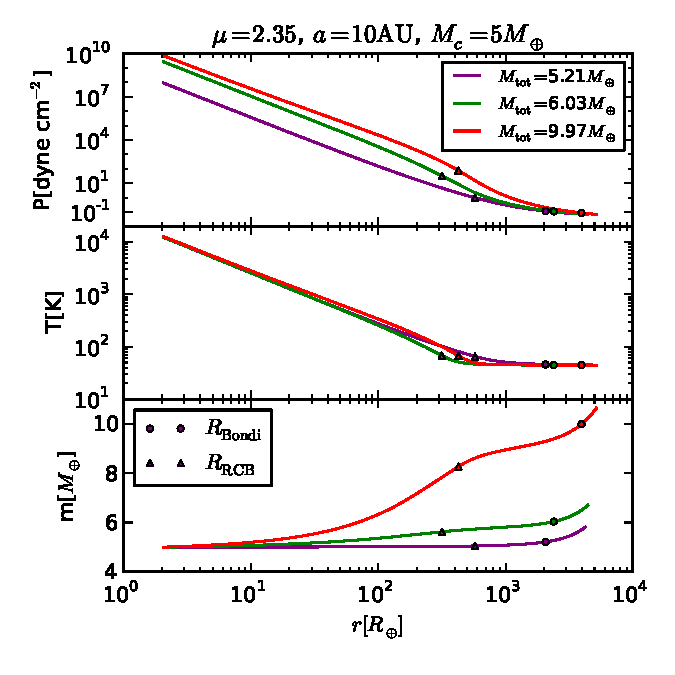
\includegraphics[width=0.5\textwidth]{../../figs/ModelAtmospheres/RadSelfGravPoly/PaperFigs/PTm_profiles_v2.pdf}
%\vspace{-0.5in}
\caption{Example pressure, temperature and total mass (core plus atmosphere) profiles as a function of radius at $a=60$ AU and for a fixed core mass $M_{\rm c}=5 M_{\oplus}$. The circles and triangles mark the locations of the Bondi radius and of the radiative-convective boundary, respectively. The solid, dotted and dashed lines correspond to profiles with total mass (core and atmosphere) of $5.12 M_{\oplus}$, $5.85 M_{\oplus}$ and $9.22 M_{\oplus}$, respectively. The 5.12 $M_{\oplus}$ and 9.22 $M_{\oplus}$ values represent the minimum and maximum total mass, respectively, that our model allows for this particular choice of disk parameters and core mass.}
\label{fig:profiles}
\end{figure}


In the initial stages of its evolution, the atmosphere is purely convective and isentropic, with an entropy equal to that of the disk. In the context of our numerical model, this is the minimum atmosphere mass for which a hydrostatic solution exists. Further gas accumulation brings in energy that has to be radiated away, and an initially thin outer radiative region forms, which becomes thicker as the atmosphere becomes more massive. 

%This layer is thin for low mass atmospheres, An increase in atmosphere mass causes the radiative zone to expand and the convective region to contract. As more and more gas is accumulated, the convective zone eventually starts expanding again; however, the ratio between the radii of the radiative and convective regions continually increases with atmosphere mass, i.e. the radiative regions of these types of atmospheres are getting deeper and deeper.  \textbf{[This needs to be rephrased, somewhat vague and repetitive.]}

%as can be seen in Fig. 1: for the $5.21 M_{\oplus}$ atmosphere, the ratio between the thickness of the radiative and convective regions is low. 

In what follows we discuss the time evolution of the envelope. We use the global cooling model developed in section \ref{cooling} to obtain an evolutionary history from series of static atmosphere profiles, using the numerical procedure described in section \ref{twolayer}. Figure \ref{fig:Ltplot} shows the luminosity evolution and the elapsed time as a function of atmosphere mass for the same choice of parameters as in Figure \ref{fig:profiles}, $a=60$ AU and $M_{\rm c}=5 M_{\oplus}$. The radiative region of the atmosphere is initially thin, which results in a relatively small number of steps that photons need to diffuse and hence a high luminosity (see equation \ref{eq:Lcb}). The luminosity decreases as the atmosphere mass grows and the radiative region becomes deeper. For comparison, we also plot the analytic results derived in section \ref{analytic}. We find only a brief agreement between the analytic and numerical results. In the early stages, the radiative zone is too shallow and the assumption that $P_{\rm RCB} \gg P_{\rm d}$ used in the analytic model breaks down. As the mass of the atmosphere grows, the neglect of self-gravity in the analytic model results in a lower luminosity (equation \ref{eq:Lcb}) and therefore a longer cooling time when compared to the numerical solution. While our analytic model does not provide an accurate quantitative description of the atmosphere evolution, we will show in section \ref{critical} that it predicts the correct scalings for the atmosphere crossover time and critical core mass.  %We see that self-gravity starts to matter 

\begin{figure}[h]
\centering
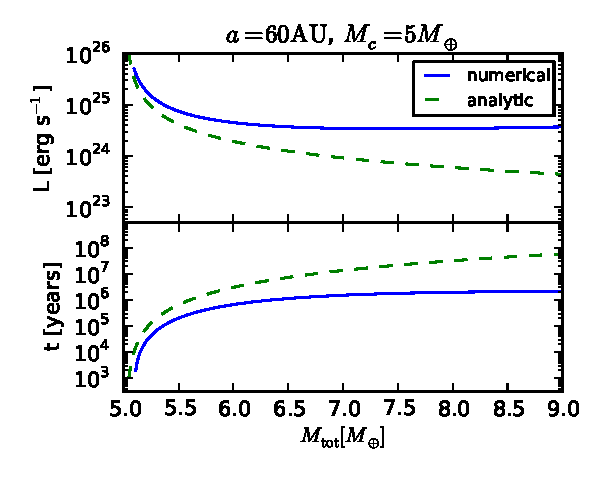
\includegraphics[width=0.5\textwidth]{../../figs/ModelAtmospheres/RadSelfGravPoly/PaperFigs/Lt_profiles_v2.pdf}
%\vspace{-0.5in}
\caption{Luminosity and time evolution of the atmosphere of a planet with fixed core mass $M_{\rm c}=5 M_{\oplus}$ and located at $a=60$ AU. The analytic result is plotted for comparison. The luminosity is initially high, then decreases as the atmosphere grows in mass and the radiative zone becomes deeper.}
\label{fig:Ltplot}
\end{figure}

 
We explain the time evolution from the bottom panel of Figure \ref{fig:Ltplot} by showing how the atmosphere growth time evolves with the atmosphere mass for a fixed core. Since the luminosity is high in the early stages, the envelope initially grows quickly; this is shown in Figure \ref{fig:growthtime} for a planet forming around a core of mass $M_{\rm c}=5 M_{\oplus}$ at several locations in our fiducial disk. Even though the atmosphere growth time, i.e. $M/\dot{M}$, is small in the early evolution stages, the increase in atmosphere mass, i.e. $\dot{M}$ is also small. As a result, the envelope spends a relatively long time at a low mass, which explains the behavior in the bottom panel of Figure \ref{fig:Ltplot}. As the radiative zone becomes thicker, the luminosity decreases and growth slows down. For $M_{\rm c}=5 M_{\oplus}$, we see that accretion is slowest for an atmosphere mass of $1-2 M_{\oplus}$. This is when the self-gravity of the atmosphere starts to matter; the envelope becomes massive enough for its energy to be large compared to the internal energy of the nebular gas. As a result, growth is continuously accelerated, and eventually runaway gas accretion settles in when the mass of the atmosphere becomes comparable to the core mass. This explains the flat behavior of the elapsed time in the later stages of the evolution, since this is when the atmosphere growth time continuously decreases, as seen in Figure \ref{fig:growthtime}. We note that in all cases presented here, growth is slowest before $M_{\rm{atm}} \sim M_{\rm c}$.  %and the estimate of the time to initiate runaway gas accretion is insensitive to the exact choice of crossover atmosphere mass to order of magnitude.
 
\begin{figure}[h]
\centering
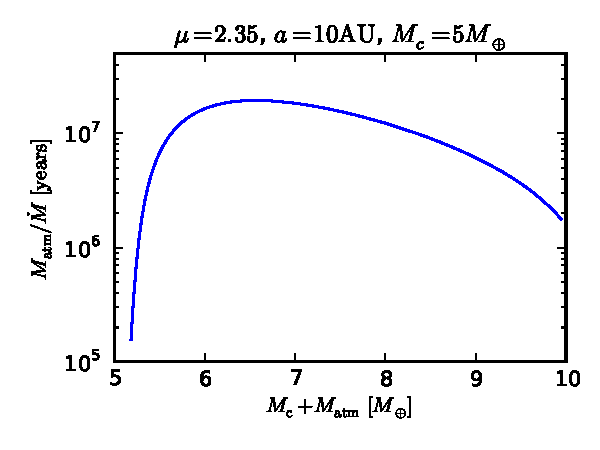
\includegraphics[width=0.5\textwidth]{../../figs/ModelAtmospheres/RadSelfGravPoly/PaperFigs/Mt_profile.pdf}
%\vspace{-0.5in}
\caption{Instantaneous growth time for the atmosphere of a planet with fixed core mass $M_{\rm c}=5 M_{\oplus}$ as a function of atmospheric mass, for a planet located at 10, 30 and 60 AU. Accretion is slowest before the mass of the atmosphere becomes comparable to the mass of the core. In this example, this happens at $M_{\mathrm{atm}} \sim 1-2 M_{\oplus}$.}
\label{fig:growthtime}
\end{figure}

The grain opacity is one source of uncertainty in our model, as it may be be lower or higher than the standard dust opacity. Dust settling or grain growth result in a lower opacity, while a high metallicity of the host star yields an enhanced opacity. Lower opacity is possible to be achieved in our regime, since we consider low planetesimal accretion rates and therefore an atmosphere that is mostly depleted of planetesimals.  A decrease in opacity reduces the number of steps that photons need to diffuse (since it increases their mean free path), resulting in a higher luminosity. In Figure \ref{fig:LtvsMopacity}, we explore opacity laws in which the coefficient $\kappa_0$ from equation (\ref{eq:opacitylaw}) is reduced by factors of 10 and 100. All things equal, a lower opacity increases the luminosity and hence speeds atmosphere growth by the same factor as the opacity reduction (see equations \ref{eq:structd} and \ref{eq:delrad}). 
 

 \begin{figure}[h]
\centering
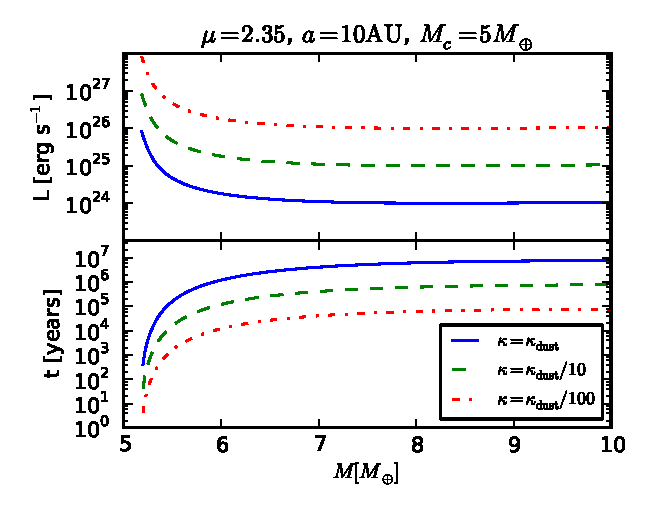
\includegraphics[width=0.5\textwidth]{../../figs/ModelAtmospheres/RadSelfGravPoly/PaperFigs/opacity_effect.pdf}
%\vspace{-0.5in}
\caption{Luminosity and time evolution as a function of atmosphere mass for planets of fixed core mass $M_{\rm c}=5 M_{\oplus}$ and located at $a=10$ AU, for different opacities. The standard dust opacity is reduced by factors of 10 and 100, respectively. A lower opacity accelerates atmosphere growth.}
\label{fig:LtvsMopacity}
\end{figure}



%\subsection{Growth Time \textbf{temporary title}}
%\label{growthtime}




\subsection{The End of Quasi-Static Evolution}
\label{endoftime}

We have shown in section \ref{profiles} that growth is continuously accelerated once the self-gravity of the atmosphere becomes important. This is due to the fact that less and less binding energy per unit of added mass is released as the envelope grows in mass, i.e. $-dE/dM$ becomes small. The right-hand side of the cooling equation (\ref{eq:coolingglobal}) is dominated by the energy loss rate $-\dot{E}$ (as we show in \App{sec:analytic}), and as a result the right-hand side of equation (\ref{eq:coolingglobal}) decreases with increasing atmosphere mass; in our calculations, we have found that it eventually becomes negative around the time when $M_{\rm{atm}} \sim M_{\rm{c}}$. This translates into a negative luminosity from the radiative-convective boundary. Physically, the luminosity $L$ represents the total heat flux through the surface defined by the radiative-convective boundary. The heat flux due to convective motions is always directed outwards and hence positive. The temperature gradient $dT/dr$ is negative, as the temperature decreases towards the outside, and the heat flux due to radiative diffusion is also positive as a result (see equation \ref{eq:structd}). This implies that, in the absence of planetesimal accretion and internal heat sources, there is no physical mechanism that can justify a negative luminosity. The quasi-static, constant luminosity approximation breaks down at this point and a more detailed, time-dependent model is necessary. However, we will show in section \ref{critical} that the existence of this unphysical result does not affect our estimates of the atmosphere evolution time or critical core mass, as the unphysical regime occurs after the slowest growth stage. %However, we have shown in section \ref{growthtime} that in all cases presented here, growth is slowest before $M_{\rm{atm}} \sim M_{\rm c}$, and the estimate of the time to initiate runaway gas accretion is therefore insensitive to the exact choice of crossover atmosphere mass to order of magnitude.



%As can be inferred from Figure 2, the time steps between subsequent evolutionary models become increasingly smaller as the atmosphere grows in mass. Around the time when the atmosphere mass is comparable to the core mass $M_{\mathrm{atm}} \sim M_{\mathrm{c}}$, we find that the time steps become negative.  

\section{Critical Core Mass}
\label{critical}

%Standard static calculations of atmosphere accretion that consider planetesimal accretion as the main source of luminosity (e.g., \citealt{mizuno78}, \citealt{stevenson82}, \citealt{rafikov06}) find that an atmosphere can be stable only if the atmosphere mass is lower than the core mass. As the mass of the envelope becomes comparable to the solid core mass, the pressure gradient can no longer balance the self-gravity of the atmosphere, and hydrostatic equilibrium breaks down. As a result, a phase of rapid gas accumulation is initiated, i.e. runaway accretion. Typically, this instability settles in when $M_{\rm{atm}} \sim M_{\mathrm{c}}$. 

 %a single value for the critical core mass $M_{\rm{crit}}$ is found, when the mass of the gaseous envelope is equal to the mass of the core. This is the maximum mass the core can have before unstable gas accretion commences. 

Standard calculations that consider planetesimal accretion as the main source of luminosity (e.g., \citealt{mizuno78}, \citealt{stevenson82}, \citealt{rafikov06}) assume a steady state at all times and find that, for a given set of disk conditions, there is a maximum mass the core can have before the onset of unstable accretion: this is defined as the critical core mass (see section \ref{intro}). In our model the atmosphere is no longer in steady state because energy balance requires gas accretion, and the atmosphere contracts on a Kelvin-Helmholtz time scale. We have shown in section \ref{profiles} that atmosphere growth is slowest before $M_{\rm{atm}} \sim M_{\rm c}$, and so the estimate of the time to initiate runaway gas accretion is insensitive to the exact choice of crossover atmosphere mass to order of magnitude. We therefore choose the effective crossover mass, past which hydrostatic balance no longer holds, to be the minimum between $M_{\rm{c}}$ and the $M_{\rm{atm}}<M_{\rm c}$ at which our model becomes unphysical according to equation (\ref{eq:dti}), noting that both of these occur after the slow accretion phase for all our parameter choices. As in section \ref{analytic}, we define the \textit{crossover time} $t_{\rm{co}}$ as the time elapsed until the atmosphere mass becomes equal to the effective crossover mass. At $t_{\rm{co}}$, runaway accretion commences.

In this section we explore the dependence of the crossover time on core, disk and gas parameters, and determine the minimum core mass needed to initiate runaway gas accretion within the lifetime of the protoplanetary disk. In section \ref{Mct} we show how the crossover time varies with core mass for fixed disk parameters, demonstrating that higher mass cores achieve runaway accretion more quickly. We explore how the crossover time is affected by by the mean molecular weight of the nebular gas in section \ref{muopacity} and by the disk temperature and pressure in section \ref{TPeffects}. Finally, we determine the minimum core mass necessary for a giant planet to form before the nebular gas dissipates in section \ref{critcore}; we define this minimum mass as the \textit{critical core mass} for runaway accretion to commence. 

%In our evolutionary model the core mass is assumed to be fixed, so the above definition for the critical core mass is not applicable. Nevertheless, we adopt a similar approach in defining the atmosphere mass past which hydrostatic balance no longer holds. We denote this mass as the minimum between the mass at which $M_{\rm{atm}}=M_{\rm{c}}$ and the mass at which the right-hand side of equation (\ref{eq:dti}) becomes negative (see section \ref{endoftime}). We therefore define the evolutionary time (or growth time, or cooling time) of the atmosphere as the time elapsed until runaway accretion commences according to the criteria above. The evolution of atmosphere mass with time is shown in Figure \ref{fig:growthtime} at several locations in the disk for a core mass $M_{\mathrm{c}}=5 M_{\oplus}$. The atmosphere instantaneous growth time, defined as $\tau=M_{\rm{atm}}/\dot{M}$, is plotted as a function of the envelope mass. We see that growth is slowest around $M_{\rm{tot}} \sim 6-7 M_{\oplus}$, after which it is continuously accelerated. The estimate of the time to initiate runaway gas accretion is therefore insensitive to the exact choice of atmosphere mass, to order of magnitude, as long as it is past the time at which accretion is slowest. %\textbf{Needs a bit of a cleanup as well.}



\subsection{Crossover Time as a Function of Core Mass}
\label{Mct}

We begin by generating atmosphere evolution profiles for cores of different masses under a fixed set of disk conditions. Figure \ref{fig:tvsM} displays $t_{\rm{co}}$ for $M_{\rm c}$ between 5 and 14 $M_{\oplus}$ at $a=10$ AU in our fiducial disk. The envelope grows faster if the core is more massive, as it can bind a gaseous atmosphere more quickly due to larger gravity. This can also be seen from the analytical results in equation (\ref{eq:tcoolan}). As such, there is a minimum core mass required to form a planet within a fixed crossover time, e.g. the typical lifetime of the protoplanetary disk, which we defined above as the critical core mass. We defer numerical estimates of the critical core mass to section \ref{critcore}.

%We also find that the atmosphere growth time is very sensitive to the core mass: for the choice of parameters in Figure \ref{fig:tvsM}, the mass increase needed to reduce the crossover time by a factor of two is only half an Earth mass. 



\begin{figure}[h]
\centering
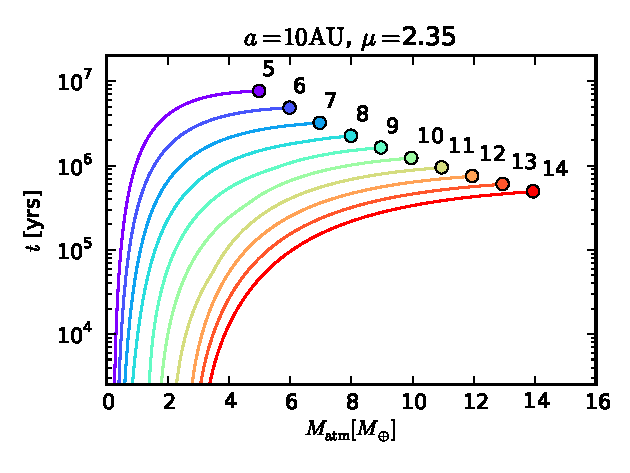
\includegraphics[width=0.52\textwidth]{../../figs/ModelAtmospheres/RadSelfGravPoly/PaperFigs/cumul_coolingtime_vs_Matm_10au_mu235.pdf}
%\vspace{-0.5in}
\caption{Time to grow an atmosphere of mass $M_{\rm{atm}}$ for cores with fixed masses between $5 M_{\oplus}$ and $14 M_{\oplus}$ at $a=10$ AU in our fiducial disk. The circles mark the crossover time where $M_{\rm{atm}} \sim M_{\rm c}$. The numbers are labeling the core mass in Earth masses. A larger core mass results in a shorter crossover time.}
\label{fig:tvsM}
\end{figure}



\subsubsection{Role of Mean Molecular Weight}
\label{muopacity}

%Figure \ref{fig:tvsMcomp} reproduces the crossover time as a function of core mass at $a=10$ AU from Figure \ref{fig:tvsM}.  

 In this work we build evolutionary atmosphere profiles assuming an ideal gas equation of state with constant mean molecular weight and adiabatic index. A realistic gas mixture, however, has variable adiabatic gradient and molecular weight, due to non-ideal effects and processes like dissociation or ionization. Future work will include realistic equation of state tables, and we expect quantitatively different results. In this study we analyze only the effect of the mean molecular weight of the nebular gas on the crossover time. In Figure \ref{fig:tvsM} we compare our standard model given by $\delad=2/7$ and $\mu=2.35$ from Figure \ref{fig:tvsM} with a model with the same adiabatic index but a different molecular mass, $\mu=2$ (i.e., purely molecular hydrogen). For comparison, we also plot the results predicted by the analytic, non self-gravitating model described in section \ref{analytic}. However, we saw in equation (\ref{eq:tcoolan}) that the crossover time as predicted by the analytic results is too long. Here we are investigating whether the analytic model predicts the correct scalings as opposed to the actual absolute results, when compared to the numerical model. We therefore estimate the analytic crossover time as the time needed for the atmosphere to reach an effective crossover mass $M_{\rm{atm}}=f M_{\rm c}$, where $f = 0.13$. The scaled analytic results are in good agreement with the numerical models. A lower mean molecular weight translates into a longer crossover time for the same core mass, since an atmosphere composed of heavier molecules has a smaller scale height, and therefore a weaker pressure gradient to oppose self-gravity.  
 


\begin{figure}[h]
\centering
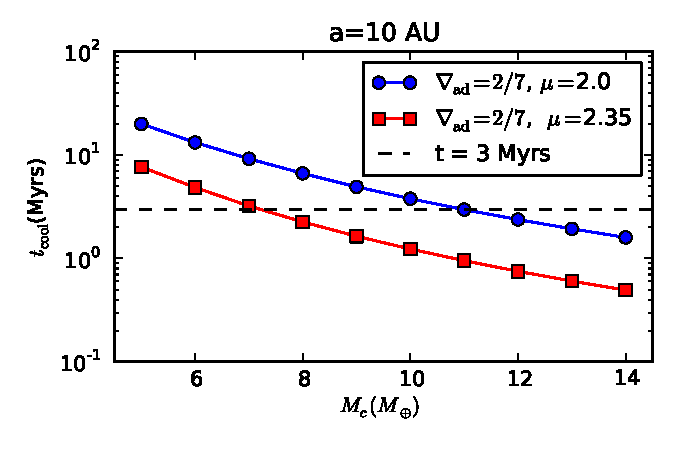
\includegraphics[width=0.48\textwidth]{../../figs/ModelAtmospheres/RadSelfGravPoly/PaperFigs/coolingtime_vs_Mc_10au.pdf}
%\vspace{-0.5in}
\caption{The crossover time $t_{\rm{co}}$ as a function of core mass at $a=10$ AU, for atmospheres with different mean molecular weight. A typical protoplanetary disk life time $t=3$ Myrs is plotted for comparison. The crossover time is larger for a lower mean molecular weight.}
\label{fig:tvsMcomp}
\end{figure}

\subsubsection{Disk Temperature and Pressure}
\label{TPeffects}
 
A planet's location in the protoplanetary disk affects its crossover time only because the disk temperature and pressure vary with stellocentric distance. Here, we study the separate effects of disk temperature and pressure on the time evolution of the atmosphere. At a fixed distance in the disk $a=10$ AU and for a core mass $M_{\mathrm{c}}=5 M_{\oplus}$, we first fix the disk pressure $P_{\rm{d}}$ at the value given by equation (\ref{eq:Pd}) and vary the disk temperature $T_{\rm{d}}$. We then fix the disk temperature at the value given by equation (\ref{eq:diskb}) and vary $P_{\rm{d}}$. The resulting variation in crossover time is plotted in Figure \ref{fig:TPeffects}. For comparison, we also plot the analytic results, using the same fractional mass scaling as in subsection \ref{muopacity}, $f=0.13$, 

\begin{figure*}[tb]
\centering
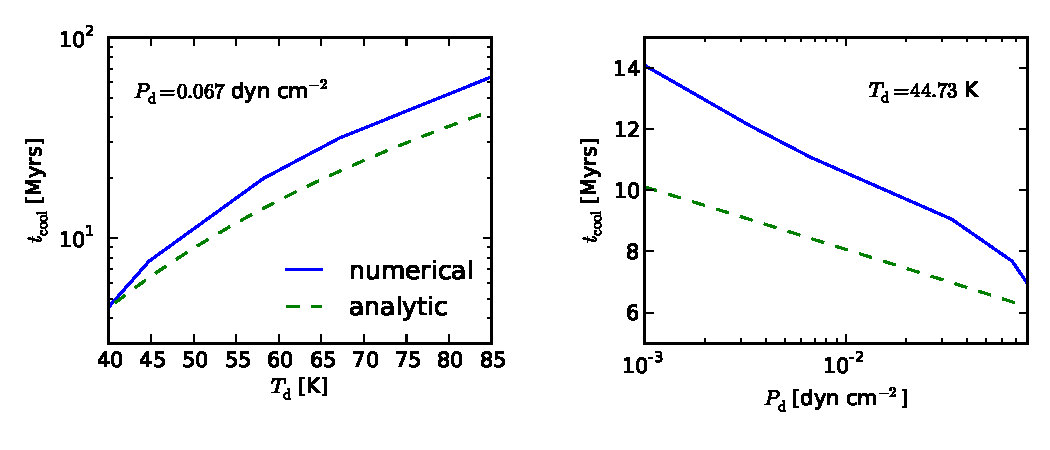
\includegraphics[width=1.\textwidth]{../../figs/ModelAtmospheres/RadSelfGravPoly/PaperFigs/TdPd_effect.pdf}
%\vspace{-0.5in}
\caption{Left panel: crossover time as a function of disk temperature for fixed disk pressure $P_{\rm d}=0.067$ dyn cm$^{-2}$ given by equation (\ref{eq:Pd}) at 10 AU and a core of fixed mass $M_{\rm c}=5 M_{\oplus}$. Right panel: crossover time as a function of disk pressure for fixed disk temperature $T_{\rm d}=44.73$ K given by equation (\ref{eq:diskb}) at 10 AU and a core of fixed mass  $M_{\rm c}=5 M_{\oplus}$. The analytic scalings are plotted for comparison, for an effective crossover mass $M_{\rm{co}}=f M_{\rm c}$ with $f=0.13$. Gas accretion is faster for lower temperatures and higher pressures.} 
\label{fig:TPeffects}
\end{figure*}

We find that the crossover time is shorter for lower disk temperatures and higher pressures. We discuss the two effects separately.

An increase in disk temperature results in a longer crossover time, as a higher temperature causes an increase in opacity. As a result, photons diffuse through the radiative layer more slowly, producing a lower planetary luminosity. Our analytic model predicts $t_{\rm{co}} \propto T^{\beta+ 1/2}$ (see equation \ref{eq:tcoolan}), where $\beta$ is the constant in the opacity law (\ref{eq:opacitylaw}). For our choice of $\beta=2$, the crossover time is therefore strongly dependent on the opacity. Different opacity assumptions will result in a different scaling with temperature of $t_{\rm{co}}$.  We note, however, that the power law dependence of the crossover time on disk temperature found in our analytic model breaks down for the numerical model for low $T\di$. Nevertheless, the trends predicted by the scaled analytic approximation in the left panel of Figure \ref{fig:TPeffects} are still informative. For the full numerical solution, a factor of $\sim 3$ reduction in the disk temperature results in an decrease of the growth time by a factor of $\sim 30$. The atmosphere evolution is therefore strongly dependent on the temperature in the protoplanetary disk.

From equations (\ref{eq:tcoolan}) and (\ref{eq:xi}), the crossover time is inversely proportional to disk pressure. A higher disk pressure therefore results in a shorter crossover time. Increasing the disk pressure by a factor of $\sim 100$ only reduces the crossover time by a factor of $\sim 2$. As such, the crossover time is only weakly dependent on the nebular pressure.

%From equation (\ref{eq:PcbRcb}), a higher disk pressure will yield the same pressure at the radiative-convective boundary $P_{\cb}$ at a larger radius of the convective zone $R_{\cb}$, and thus at a larger atmosphere mass from equation (\ref{eq:Matman}). A higher mass implies the atmosphere will become critical on a shorter timescale.


 %This effect is likely due to the fact that a higher disk pressure, and hence density, leads to the atmosphere becoming self-gravitating and therefore initiating runaway accretion on a faster timescale. However, increasing the disk pressure by a factor of $\sim 100$ only reduces the atmosphere growth time by a factor of $\sim 2$. As such, the atmosphere cooling time is only weakly dependent on the nebular pressure.

%\begin{figure}[h]
%\centering
%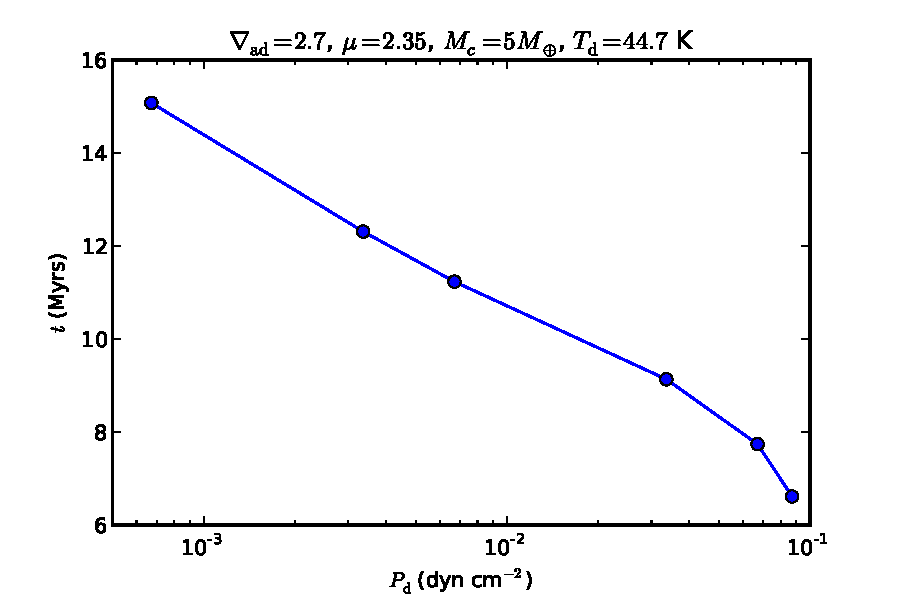
\includegraphics[width=0.5\textwidth]{../../figs/ModelAtmospheres/RadSelfGravPoly/PaperFigs/Pd_effect.pdf}
%%\vspace{-0.5in}
%\caption{Disk pressure effect on growth time. Gas accretion is faster for higher pressures.}
%\end{figure}

%In contrast with the pressure effect, an increase in disk temperature causes the growth time to increase as well. This is due to opacity effects: a higher disk temperature increases the opacity in the radiative zone of the atmosphere, causing a decrease in luminosity and therefore a longer Kelvin-Helmholtz accretion time. Moreover, a factor of $\sim 3$ reduction in the disk temperature results in an decrease of the growth time by a factor of $\sim 30$. The atmosphere evolution is therefore strongly dependent on the temperature in the protoplanetary disk. %We also notice that the analytic scaling is 





\subsection{Critical Core Mass}
\label{critcore}

We can now combine the results obtained in section \ref{Mct} to determine the minimum core mass necessary for a protoplanet to initiate runaway gas accretion within the disk lifetime, i.e. to have a crossover time less than the disk lifetime. We  denote this mass the \textit{critical core mass}.

%In the previous subsections we explored the effect of disk and gas properties on the growth time of an atmosphere accreting around a protoplanetary core of fixed mass. The main question we address here is under what conditions the atmosphere can grow before the gas in the protoplanetary disk is dissipated. Specifically, we determine the minimum core mass that is necessary for a protoplanet to initiate runaway gas accretion within the disk lifetime, i.e. to have a crossover time equal to the disk life timescale. We  denoted this mass the \textit{critical core mass} in section \ref{Mct}.

Observations of protoplanetary disks show that they dissipate over a time scale of a few million years (e.g., \citealt{lagrange00}, \citealt{haisch01}, \citealt{goldreich04}). We adopt a disk life timescale of $\tau=3 $ Myrs and determine the critical core mass as a function of disk temperature, pressure and mean molecular weight of the nebular gas. 

\begin{figure}[h]
\centering
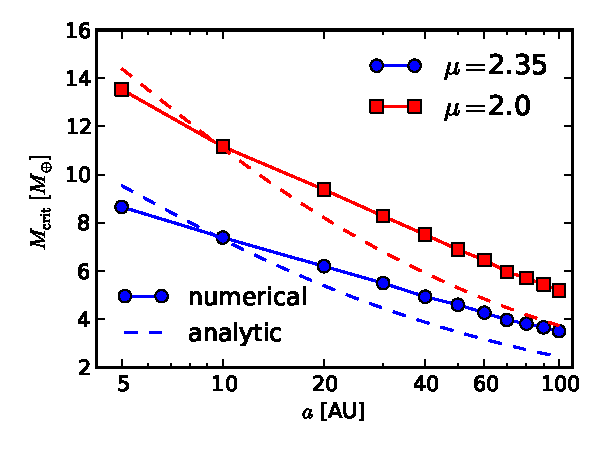
\includegraphics[width=0.5\textwidth]{../../figs/ModelAtmospheres/RadSelfGravPoly/PaperFigs/Mcrit_vs_a_3Myrs_new.pdf}
%\vspace{-0.5in}
\caption{The minimum core mass for an atmosphere to initiate runaway gas accretion within the lifetime of a typical protoplanetary disk $t \sim 3$ Myrs as a function of semi-major axis, for different mean molecular weight of the nebular gas. The analytic scaled results are plotted for comparison. The critical core mass is lower at larger stellocentric distances.}
\label{fig:Mcvsa}
\end{figure}

 In Figure \ref{fig:Mcvsa}, we see that the critical core mass decreases for larger separations, primarily due to the fact the disk temperature is lower in the outer regions of the disk. As we showed in section \ref{Mct}, the atmosphere grows faster for lower temperatures, which offsets the need for a larger core mass. The critical core mass is larger for a lower mean molecular weight, consistent with the results derived in section \ref{Mct}. We also explore the opacity effect on the critical core mass in Figure \ref{fig:Mcritopacity}. For an opacity, and therefore crossover time, that is an order of magnitude larger, the critical core mass is increased by roughly a factor of 2. 

%The comparison between our results and standard values for the critical core mass due to planetesimal accretion is deferred to section \ref{acc}.  % \textbf{Need to add qualitative explanations for different slopes and curve intersection}
%
%\subsection{Opacity Dependence}
%\label{opacity}
% 
% In this section we investigate the effect of opacity reduction on the atmosphere evolution. We explore opacity laws in which in which the constant $\kappa_0$ from equation (\ref{eq:opacitylaw})  is reduced by factors of 10 and 100. The result is depicted in Figure \ref{fig:LtvsMopacity}. All things equal, a lower opacity increases (decreases) the luminosity (cooling time) by the same factor as the opacity reduction (see equations (\ref{eq:structd}) and (\ref{eq:delrad})). 
% 
%
% \begin{figure}[h]
%\centering
%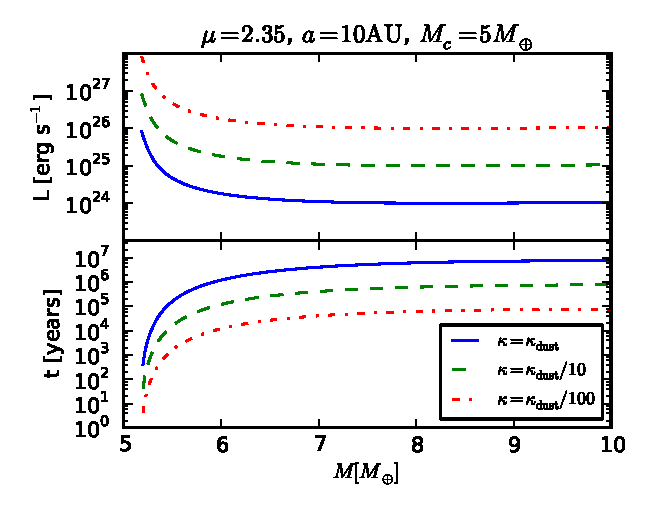
\includegraphics[width=0.5\textwidth]{../../figs/ModelAtmospheres/RadSelfGravPoly/PaperFigs/opacity_effect.pdf}
%%\vspace{-0.5in}
%\caption{Comparison between standard dust opacity and opacity reduced by factor of 10 and 100, respectively. Lower opacity accelerates atmosphere growth.}
%\label{fig:LtvsMopacity}
%\end{figure}



\begin{figure}[h]
\centering
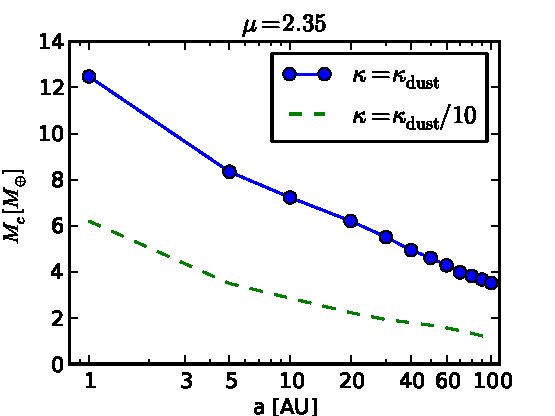
\includegraphics[width=0.5\textwidth]{../../figs/ModelAtmospheres/RadSelfGravPoly/PaperFigs/Mcrit_vs_a_3Myrs_opacity.pdf}
%\vspace{-0.5in}
\caption{Critical core mass as a function of semi-major axis for different opacities. A factor of ten opacity reduction results in a critical core mass twice as small.}
\label{fig:Mcritopacity}
\end{figure}

%\section{Discussion}
%\label{discussion}
%
%In this section we discuss the parameter space of validity of our model. We calculate the conditions under which planetesimal accretion can be ignored, and review the effects of some of the approximations that come into our model.


 
 \section{Neglected Effects}
 \label{neglected}
 
 In this section we summarize some of the simplifications we have made, and discuss future work.
  
 \subsection{Planetesimal Accretion}
 
 %In this study we explore the formation of giant planets through core accretion under the assumption that the protoplanetary core is already fully formed and the planetesimal accretion rate is low. 
 
 Standard calculations in which the atmosphere evolution is dominated by planetesimal accretion find that the critical core mass to form a giant planet is of the order of $10 M_{\oplus}$. We have showed in Figure \ref{fig:Mcvsa} that our calculations yield lower critical core masses even in the more inner parts of the disk for a gas with standard composition. It is therefore easier, to first order, to first form the core, then lower planetesimal accretion and accumulate a massive atmosphere. We defer concrete quantitative comparisons between our values and standard results to Piso et al. (2013, in prep). 
 
 \subsection{Equation of State}
 \label{EOS}
 
 In our model we assume an ideal gas law and a polytropic equations of state (EOS), given by equations (\ref{eq:idealgas}) and (\ref{eq:polyEOS}), respectively. However, non-ideal effects such as partial dissociation and ionization have to be taken into account. One solution is using tabulated equation of state tables for hydrogen and helium mixtures. As future work, we plan to use the \citet{saumon95} EOS tables and extend them to lower pressures and temperatures as required by our disk assumptions.
 
 \subsection{Time Evolution}
 
 In this study we have assumed that the luminosity stays constant throughout the radiative region of the atmosphere. As a result, the time dependence can be neglected in equation (\ref{eq:structd}) and static solutions can be obtained and then connected through a global cooling equation, as described in section \ref{cooling}. However, the assumption of constant luminosity breaks down for high atmosphere masses, as described in section \ref{endoftime}; in this case, a time-dependent model is required to describe the atmosphere evolution. We are currently developing a full evolutionary time-dependent atmosphere model. We do not expect qualitatively different results. We showed in section \ref{endoftime} that the quasi-static model breaks down around the time when the atmosphere mass becomes equal to the mass of the core. Nevertheless, we can see from Figure \ref{fig:growthtime} that accretion is slowest before the region in which our model breaks down, and hence the time to initiate runaway gas accretion is insensitive to the exact choice of atmosphere mass at which this process starts. As a result, we are confident of our results to order of magnitude.
 
% \subsection{Inefficient Convection}
 
%\textbf{Discussion about mixing length theory...} 

%\subsubsection{Opacity \textbf{(Paper II)}}

%\textbf{In progress, still need to run models for smaller AU and see at what point ice grain opacity is no longer valid. Currently strange behavior at 1 AU for $\delad=2/5$, the critical core mass goes up significantly instead of having a linear trend. $\delad=2/7$ atmospheres do not show this effect. Models for the inner disk would also show / confirm that close-in giant planet formation is hard (need larger core mass).}
 
 
 \section{Summary}
 \label{conclusions}
 
 In this paper we have studied the formation of giant planet atmospheres under the assumption of a low planetesimal regime in which Kelvin-Helmoholtz gas contraction dominates the luminosity evolution of the atmosphere. We built quasi-static two-layer atmosphere models with an inner convective region and an outer radiative region that matches smoothly onto the protoplanetary disk at the Hill radius. In our static models, we used an ideal gas polytropic equation of state, and assumed a standard ISM power-law opacity. We then derived a cooling model to connect series of quasti-static atmospheres, and thus obtained an evolutionary history of the envelope. We defined the time $t$ at which unstable atmosphere collapse commences as the \textit{crossover time} $t_{\rm{co}}$, for which $M_{\rm atm}(t_{\rm{co}})\sim M_{\rm c}$. From this we defined as \textit{critical core mass} the minimum core mass for a protoplanet to initiate runaway gas accretion during the lifetime of the protoplanetary disk. We studied this minimum mass for a variety of disk conditions, nebular gas compositions and opacities. We found that the critical core mass decreases for lower disk temperatures, and hence for larger stellocentric distances. Moreover, we found that an opacity reduction also lowers the critical core mass significantly. On the other hand, a lower mean molecular weight of the nebular gas results in a larger critical core mass.
  
 We also find that the critical core mass to form a giant planet within the life time of the disk (of about 3 Myrs) is smaller than the typical 10 $M_{\oplus}$ value yielded by studies that assume that the atmosphere evolution is dominated by the luminosity due to planetesimal accretion. As such, it is faster to form a planet by growing the core first in a fast planetesimal accretion regime (e.g., the core forms in the inner disk, then migrates outwards), then significantly reduce planetesimal accretion and allow a massive atmosphere to accumulate. 
 
%Our study assumes that the protoplanetary core forms first, then it r
 
%---------------------------------------------------------------------------
\bibliographystyle{apj}
\bibliography{refs}

\appendix
\section{Derivation of Global Energy Equation}\label{sec:virial}

We derive here the global energy equation (\ref{eq:coolingglobal}).  We follow the simpler example in \S4.3 of \citet{kippenhahn90}, adding the effects of finite core radius, surface pressure and mass accretion.  We assume that hydrostatic balance holds.  Integrating the local energy equation (\ref{eq:structd}) from core to surface gives:
\begin{subeqnarray}
\label{eq:coolinglocal}
L - L\co &=& \int_{M\co}^M {\p L \over \p m} dm \\
&=& \int_{M\co}^M \left(\epsilon - T {\p S \over \p t} \right)dm \\
&=& \Gamma  - \int_{M\co}^M{\p u \over \p t} dm +  \int_{M\co}^M {P \over \rho^2} {\p \rho \over \p t} dm\slabel{eq:DLc}\, .
\end{subeqnarray} 
with $\Gamma \equiv \int \epsilon dm$ the rate of intern heat generation.

In what follows, we must carefully distinguish between partial time derivatives, $\p / \p t$, (performed at fixed mass) and total time derivatives, denoted with overdots (which include the effect of mass accreted through the outer boundary). % or $d/dt$.  
For instance, the surface radius $R$ evolves as  
\begin{equation}\label{eq:Rdot}
 \dot{R} = {\p R \over \p t} + {\dot{M} \over 4 \pi R^2 \rho\surf}
\end{equation} 
where $\p R/\p t$ gives the Lagrangian contraction of surface mass elements, and $\dot{M}$ denotes mass accretion rate through the upper boundary.  The subscript $M$  denotes quantities at the upper boundary of total mass $M$ (though it is omitted from $M$ and $R$).  Similarly the volume, $V = (4 \pi/3)r^3$ and pressure at the surface evolve as
\begin{subeqnarray}\label{eq:dot}
\dot{V}_M &=&  {\p V_{\rm M} \over \p t} + {\dot{M} \over \rho_{\rm M}}  \\
 \dot{P}_M &=& {\p P_{\rm M} \over \p t} + {\p P_M \over \p m}\dot{M} \\
 &=&  {\p P_{\rm M} \over \p t} - {G M  \over 4 \pi R^4} \dot{M}\, .
\end{subeqnarray} 
For the purpose of this derivation we will hold the core mass fixed $\dot{M}\co = 0$ which further gives $\dot{P}\co = \p P\co / \p t$.

To derive the global energy equation (\ref{eq:coolingglobal}) we must move the (partial) time derivatives in \Eq{eq:DLc} outside their integrals.  The internal energy integral follows simply from  Leibniz's rule as
\begin{equation}\label{eq:udot}
\int_{M\co}^{M(t)}{\p u \over \p t} dm = \dot{E}_i  -  \dot{M}u\surf\, .
\end{equation} 

To evaluate the work integral, we derive a pair of expressions for the rate of change of gravitational energy.
The time derivative of \Eq{eq:virial}  gives
\begin{eqnarray}\label{eq:EGdot}
\dot{E}_G &=& 3  \int_{M\co}^M {P \over \rho^2} {\p \rho \over \p t} dm -3 \int_{M\co}^M {\p P\over \p t}{dm \over \rho} \\
&& -  3{P\surf \over \rho\surf} \dot{M}+ 3 \dot{P}\surf V\surf -3 \dot{P}\co V\co  + 3  P\surf {\dot{ V}\surf} \, . \nonumber
%&&+ 4 \pi \left. \left(r^3 {\p P \over \p t}\right)\right|_{M\co}^M  + 3  P\di {\p V \over \p t}  - {G M \over R} \dot{M} \nonumber
\end{eqnarray} 
%where the volumes, $V\surf = 4 \pi R^3/3$ and $V\co = 4 \pi R\co^3/3$. 
The first integral in \Eq{eq:EGdot} is the one we want, but the next one must be eliminated.  The time derivative of \Eq{eq:Eg} (times four) gives
\begin{subeqnarray}
 4 \dot{E}_G &=&  -4 {G M \dot{M} \over R} + 4 \int_{M\co}^M {G m \over r^2}{\p r \over \p t} dm\\ 
&=&   -4 {G M \dot{M} \over R} + 4 \pi \int_{M\co}^M r^3{\p \over \p m}{\p P \over \p t} dm \slabel{eq:4EGb} \\
&=&  -4 {G M \dot{M} \over R} -3  \int_{M\co}^M {\p P\over \p t}{dm \over \rho} \slabel{eq:4EGc} \\
&&+ 3 V\surf {\p P\surf \over \p t} -3 V\co {\p P\co \over \p t} \nonumber 
\end{subeqnarray} 
where \Eqs{eq:4EGb}{eq:4EGc} use hydrostatic balance  and integration by parts.

%To eliminate the time derivates of pressure, we take the time derivative of the hydrostatic balance equation for $\p^2 P / \p m\p t$ and integrate over $4\pi r^3 dm$ (as in the virial equation derivation) to get
%\begin{equation}\label{eq:dHBdt}
%3 \dot{P}\surf V\surf -3 \dot{P}\co V\co -3 \int_{M\co}^M {\p P\over \p t}{dm \over \rho}  = 4 \dot{E}_G + 4{G M \over R} \dot{M}  \, .
%\end{equation} 
%Combining \Eqs{eq:EGdot}{eq:dHBdt} gives 
%\begin{eqnarray}\label{eq:rhodot}
%\int_{M\co}^M {P \over \rho^2} {\p \rho \over \p t} dm  &=& - \dot{E}_G - {4 \over 3}{G M\over R} \dot{M} + {P\surf \over \rho\surf} \dot{M} -  P\surf \dot{V}\surf  \, , \nonumber \\
%&=&- \dot{E}_G - {4 \over 3}{G M\over R} \dot{M}  -  P\surf {\p V\surf \over \p t}  \, ,
%\end{eqnarray} 
%where the final step uses \Eq{eq:Rdot}.

Subtracting \Eqs{eq:udot}{eq:4EGc} and rearranging for the desired integral gives
\begin{eqnarray}\label{eq:PdVint}
\int_{M\co}^M {P \over \rho^2} {\p \rho \over \p t} dm  &=&  - \dot{E}_G - {G M \dot{M} \over R} - P\surf {\p \dot{V}\surf \over \p t} \,  
\end{eqnarray} 
with \Eq{eq:dot} used to combine terms.  Combining \Eqsss{eq:DLc}{eq:udot}{eq:PdVint}, we reproduce \Eq{eq:coolingglobal} with the accreted energy $e_{\rm acc} \equiv u\surf - GM/R$.  

%\begin{figure}[tb]
%\centering
%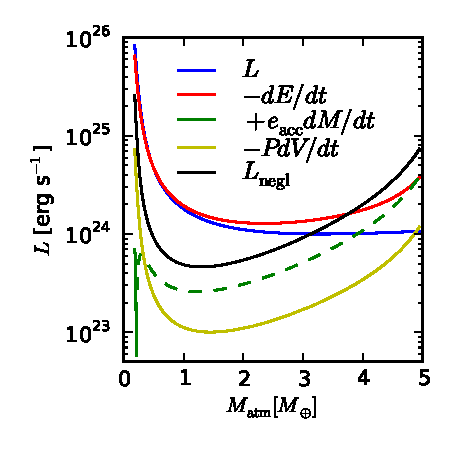
\includegraphics[width=0.5\textwidth]{../../figs/ModelAtmospheres/RadSelfGravPoly/PaperFigs/cooling_a10_Mc5_rcb.pdf}
%%\vspace{-0.5in}
%\caption{}
%\end{figure}



\section{Analytic Cooling Model Details}\label{sec:analytic}

\subsection{Isothermal Atmosphere}
\label{iso}

We consider the structure of a low mass non self-gravitating isothermal atmosphere.  We assume the atmosphere matches onto a constant background density, $\rho_{\rm d}$, at a distance $r_{\rm fit} = n_{\rm fit} \RB$, where $R_{\rm B}$ is the Bondi radius defined in equation (\ref{eq:RB}). From equation (\ref{eq:structa}) the resulting density profile is
\begin{equation} \label{eq:rhoiso}
\rho = \rho_{\rm d} \exp \left({R_{\rm B} \over r} - {1 \over n_{\rm{fit}}} \right) \approx   \rho_{\rm{d}} \exp \left(R_{\rm B} \over r  \right),
\end{equation} 
where the approximate inequality is valid deep inside the atmosphere ($r \ll \RB$) for any $n_{\rm fit} \gtrsim 1$.  However, the choice of boundary condition does have an order unity effect on the density near the Bondi radius. 

The mass of the atmosphere is determined by integrating equation (\ref{eq:structb}) from the core to the Bondi radius using the density profile (\ref{eq:rhoiso}).  Planets can attract massive atmospheres if $\theta\co \equiv R_B/R\co \gg 1$.  In this case
\begin{equation} \label{eq:MatmISO}
M_{\rm iso} \approx 4 \pi \rho\di {R\co^4 \over R_B} e^{R_B/R\co} = 4 \pi \rho\di {R\co^3 \over \theta\co} e^{\theta\co}\, .
\end{equation} 
This result is the leading order term in a series expansion.  Furthermore, because the atmospheric scale-height at $R\co$ is $H_\rho = |dr /d\ln\rho| = R\co^2/R_B$, the result is intuitively the correct order of magnitude.

\subsection{Temperature and Pressure Corrections at the Radiative-Convective Boundary}
\label{RCBcorr}

%\subsection{Temperature Contrast at Convective Boundary}
In this section we estimate the temperature and pressure corrections at the radiative-convective boundary due to the fact that the radiative region is not purely isothermal. We show that the temperature contrast between the temperature at the radiative-convective boundary $T_{\rm RCB}$ and the ambient disk $T_{\rm d}$, is modest.  From equation (\ref{eq:delrad}), we express the radiative lapse rate
\begin{equation}\label{eq:delradan}
\delrad = {3 \kappa P \over 64 \pi  G M \sigma T^4} L = \nabla\di {(P/P_{\rm d})^{1+\alpha} \over (T/T_{\rm d})^{4-\beta}},
\end{equation}

\noindent where the second equality follows from the opacity law (\ref{eq:opacitylaw}), and $\nabla_{\rm d}$ is the radiative temperature gradient at the disk:

\begin{equation}
\label{eq:delo}
\nabla \di \equiv \frac{3 \kappa(P{\di}, T{\di}) P{\di}}{64 \pi G M \sigma T_{\rm d}^4} L.
\end{equation}

\noindent The mass $M$ is the sum of the core mass and the atmosphere mass below the pressure level $P$.  If the mass in the radiative zone is small, then we can hold $M$ fixed at the sum of the core and convective zone masses: $M = M\co + M_{\cb}$.   With this assumption, we get a constant value for $\nabla_{\rm d}$.  As $\delrad=d \ln T/d \ln P$, the temperature profile integrates to
\begin{equation}\label{eq:radTP}
\left(T \over T_{\rm d}\right)^{4-\beta} - 1 = {\nabla\di \over \nabla_\infty} \left[\left({P \over P_{\rm d}}\right)^{1+\alpha} - 1 \right] \, ,
\end{equation} 
where $\nabla_\infty = (1+\alpha)/(4-\beta)$ is the radiative temperature gradient for $T ,P \rightarrow \infty$.
By applying \Eqs{eq:delradan}{eq:radTP} at the radiative-convective boundary (where $\delrad = \delad$) under the assumption that the pressure there $P\cb$ satisfies the relation $P\cb \gg P_{\rm d}$, we end up with the expression in equation (\ref{eq:Tcb}), $T\cb=\chi T\di$, with $\chi$ defined in equation (\ref{eq:chi}).

 . %\begin{equation}\label{eq:Tcb}
%\chi \equiv {T\cb\over T_{\rm d}} \simeq \left(1 - {\nabla_{\rm ad} \over \nabla_\infty}\right)^{-\frac{1}{4-\beta}} \, .
%\end{equation} 
%For  $\alpha=0$ and $\beta =2$,  and assuming $\delad = 2/7$, we find $\chi \approx 1.5$. Values of $\chi$ and $\nabla_\infty$ for other choices of $\beta$ are summarized in \App{sec:analytic}.

%\footnote{Our definitions of $\nabla\di$ and $\nabla_\infty$ are precisely opposite to \citet{rafikov06}, but consistent with other works and the general convention of labeling a quantity $f$ in the disk as $f\di$.}

The pressure at the convective boundary  follows from \Eqs{eq:radTP}{eq:Tcb} as
\begin{equation}
\label{eq:Pcbapprox}
{P\cb\over P_{\rm d}} \simeq \left({\delad/\nabla\di \over 1 - \delad/\nabla_\infty}\right)^{1 \over 1 + \alpha}
\end{equation} 
This pressure contrast can be quite large since $\nabla_{\rm d} \ll 1$.
 
 We now eliminate $\nabla\di$ from equation (\ref{eq:Pcbapprox}) to obtain a relation between temperature and pressure as a function of the pressure at the radiative-convective boundary $P\cb$. From equation (\ref{eq:radTP}), it follows that
 \begin{equation}\label{eq:TP}
{T \over T_{\rm d}} = \left\{1 + {1 \over {\nabla_\infty \over \delad} - 1} \left[ \left({P \over P\cb}\right)^{1+\alpha} -  \left({P_{\rm d} \over P\cb}\right)^{1+\alpha}  \right] \right\}^{1 \over 4-\beta}\, .
\end{equation} 
 We can then determine the radius of the convective boundary $R\cb$ from the hydrostatic balance equation (\ref{eq:structa}) as 
\begin{equation}\label{eq:RCBint}
{R_B \over R\cb} = \int_{P\di}^{P\cb} {T \over T_{\rm d}} {dP \over P}\, .
\end{equation} 
An isothermal atmosphere gives a simple logarithmic dependence on $P\cb$.  However, using \Eq{eq:TP} in the integral gives
\begin{equation}\label{eq:Rcb}
{R_B \over r\cb} = \ln \left(P\cb \over P\di \right) - \ln \theta \, ,
\end{equation} 
with an extra correction term, $\theta < 1$.  From this we arrive at the relation between $P\cb$ and $P\di$ given by equation (\ref{eq:PcbRcb}).

% The form we chose for the correction term allows us to relate the disk and radiative-convective boundary pressures as :
% \begin{equation}\label{eq:PcbRcb}
%P\cb = \theta P_{\rm d} e^{R_B/R\cb} \, .
%\end{equation}   
%In the $P\cb \gg P_{\rm d}$ limit, the correction term is an order unity constant that depends on $\alpha$, $\beta$ and $\delad$. Similarly to the temperature correction factor $\chi$,  $\theta$ accounts for the fact that the radiative region is not perfectly isothermal. For $\delad=2/7$, $\alpha=0$ and $\beta=2$, we find $\theta \approx 0.556$. Values of $\theta$ for other choices of $\beta$ are summarized in \App{sec:analytic}.  A simple analytic expression for $\theta$ is not possible.  


\subsection{Estimate of Atmosphere Mass Outside the Bondi Radius}

Here we consider the mass exterior to the Bondi radius.  For a meaningful evaluation we only include the mass coming from the overdensity relative to the background density.  The resulting external mass for an isothermal atmosphere is
\begin{subeqnarray}
M_{\rm ext} &=& 4 \pi \int_{\RB}^{r_{\rm fit}} (\rho - \rho\di) r^2 dr \\
&=& M\co \theta\co \int_1^{n_{\rm fit}} 3 \left[ \exp \left({1 \over x} - {1 \over n_{\rm fit}}\right) - 1 \right] x^2 dx  \nonumber \\
&\equiv& M\co \theta\co I(n_{\rm fit})
\end{subeqnarray} 
where $\theta_c=R_B/R_{\rm c}$ and the dimensionless integral $I(n_{\rm fit})$ obeys the limits $I(1) = 0$ and $I \rightarrow n_{\rm fit}^2/2$ as $n_{\rm fit} \rightarrow \infty$.  Since this external mass does not converge, the choice of an outer boundary does matter in principle.  In practice, however, the assumption that   $r_{\rm fit} = R_{\rm H}$ limits $n_{\rm fit}$ to modest values
\begin{equation}
n_{\rm fit} = {R_{\rm H} \over \RB} \approx 1.3 {\aun{10}^{4/7} \over \mcn{10}^{2/3}}{F_T \over  m_\ast^{1/3}}.
\end{equation} 
Since for instance $I(2) = 1.1$, these modest $n_{\rm fit}$ values will only produce a small external mass.


\subsection{The Opacity Effect}
A  lower opacity  could lower the core mass.  Reducing the opacity by a factor of one hundred cuts the core mass by more than a factor of 10, specifically to 9 $M_\oplus$ for the parameters in \Eq{eq:Mcrit}.  The reduction is not  as strong as the nominal scaling would imply, $0.01^{3/5} \approx 0.06$, because $\xi$ increases.

Even with significantly lower opacities, radiative diffusion remains a good approximation at the radiative-convective boundary.  We estimate the optical depth as (for $\beta = 2$):
\begin{equation}
\tau\cb \sim {\kappa P\cb \over g} \sim 7 \times 10^4 {F_T^4 F_\kappa \over \left(\mc \over 10 \right) \left(\au \over 10\right)^{12 \over 7}} 
\end{equation} 
where $P\cb \sim P_M$ for a self-gravitating atmosphere and $g \sim G M\co/R_B^2$, with both approximation good to within the the order unity factor $\xi$.  Clearly $\tau\cb \gg 1$ even for $F_\kappa \lesssim 0.01$ out to very wide separations.

A hotter disk would increase core masses.  Instead of our passive disk model, adopting the standard Hayashi temperature profile would increase core masses by $\sim 50\%$.  A hotter accretion phase would further increase core masses, but such phases are presumably short lived.

\subsection{Surface Terms}
We now check the relevance of the neglected surface terms in \Eq{eq:coolingglobal}.  We already showed that accretion energy can be exactly eliminated by choosing an outer boundary near the Bondi radius.   We now show that accretion energy is also a small correction at the RCB.   A rough comparison, (ignoring terms of order $\xi$) of  accretion luminosity vs.\ $\dot{E}$ gives
\begin{equation}
{G M \dot{M} \over R \dot{E}} = {G M  \over R}{dM \over dE} \sim {G M\co^2 \over R_B E}{P\cb \over P_M} \sim \sqrt{R\co \over R_B} \ll 1,
\end{equation} 
where we assume $P\cb \sim P_M$  for a massive atmosphere.  Accretion energy at the protoplanetary surface is thus very weak for marginally self-gravitating atmospheres, and even weaker for lower mass atmospheres.  A similar scaling analysis shows that the work term, $P\surf \p V\surf/\p t$ is similarly weak.  Nevertheless our numerical calculations include these surface terms in a more realistic and complete model of self-gravitating atmospheres.


\subsection{Hydrogen Dissociation}
The dissociation of molecular hydrogen deep in the atmospheres of accreting protoplanets plays a significant role in the energetics of core accretion.  In the high density regions $r  \ll R\cb$ of a convective atmosphere, the thermal plus gravitational energy scales as
\begin{equation}
dE = -4 \pi \nabla_{\rm ad}^{1/\nabla_{\rm ad}} \rho\cb R_B'^{1/(\gamma-1)} r^{\frac{2\gamma - 3}{\gamma - 1}} {dr \over r}
\end{equation} 
If $\gamma < 3/2$ then the main contribution to the energy is at the bottom of the atmosphere, i.e.\ the core.  This is the case for a diatomic ideal gas ($\gamma = 1.4$) or a solar mixture of hydrogen and helium ($\gamma \approx 1.43$).  However a monatomic gas has $\gamma = 5/3 > 3/2$.  In this case, the atmosphere's energy is no longer concentrated near the bottom, but will be concentrated near the top of the convective zone.

A likely structure is an atmosphere that is dissociated near the base, but becomes molecular near the top of the convective zone.  In this case the atmosphere's energy budget would be concentrated near the atomic to molecular transition.

The energy required to dissociate a hydrogen molecule, $I = 4.467$ eV can be significant to the overall energy budget.
Since
\begin{equation}
{I \over \nabla_{\rm ad} G M\co (2 m_{\rm H})/r} \approx 3 \left(M\co \over 10 M_\oplus \right)^{-2/3} {r \over R_{\rm c}}
\end{equation} 
we see that this energy is always relevant.

We can use the Saha equation to determine where dissociation is significant,
\begin{equation}
{n_{\rm H}^2 \over n_{\rm H_2}} = \left(\pi m_{\rm H} k T \over h \right)^{3/2} e^{-I/(kT)}
\end{equation} 
We introduce a reaction coordinate $\delta$ so that $n_{\rm H} = 2 \delta n_o$ and $n_{\rm H_2} = (1-\delta) n_o$ with $n_o = \rho X/(2 m_{\rm H})$ the number density when all hydrogen is molecular.  We express equilibrium as
\begin{equation}
{\delta^2 \over 1-\delta} = f_\mu {P_{\rm diss}(T) \over P}
\end{equation} 
with the characteristic pressure below which dissociation occurs is
\begin{equation}
P_{\rm diss} = {\left(kT\right)^{5/2} \over 4} \left( \pi m_{\rm H} \over h^2\right)^{3/2}  e^{-I/(kT)}
\end{equation} 
and the order unity factor
\begin{equation}
f_\mu = 2\delta + (1-\delta) + Y/2 + Z/\mu_Z
\end{equation} 
accounts for variations in the mean molecular weight with dissociation.  (Take $\mu_Z = 31/2$, but not too significant.)

Thus dissociation occurs where $P \lesssim P_{\rm diss}(T)$.  At disk temperatures (say 150 K) the dissociation pressure is negligibly small ($\sim 10^{-141}$ dyne cm$^{-2}$) and no dissociation occurs.  However at core temperatures the dissociation pressure is quite large especially for massive cores.  Dissociation is guaranteed.


\begin{deluxetable}{cccccc}  % <--- column justification (center/left/right)
\gdef \numcols {6}
\tablecolumns{\numcols}
\tablecaption{Parameters Describing Structure of Radiative Zone.}
\tablehead{   \multicolumn{\numcols}{c} {$\gamma = 7/5$ ($\delad = 2/7$), $\alpha = 0$} }  
\startdata
 $\beta$   		 &1/2  	& 3/4 &1   		& 3/2  		& 2   \\
 $\nabla_\infty$ & 2/7 \tablenotemark{a}  	&  4/13	& 1/3 	& 2/5 	 	& 1/2 \\
 $\chi$ 		 & \nodata &  2.25245 &1.91293 	& 1.65054 	& 1.52753 \\
 $\theta $  		 &\nodata   & 0.145032	&0.285824   &0.456333   & 0.556069   \\
\enddata
\tablenotetext{a}{Since $\delad = \nabla_\infty$ there is no convective transition at depth for this case.}
\end{deluxetable}


\end{document}

% We then apply the model to one particular super Earth, GJ 1214 b, and generalize it for all super Earths. We summarize our results and findings in the next paragraphs. 

%First, we modeled the planetary magnetic field as a dynamo (section \ref{dynamo}). We then presented a model of the magnetic interaction between a super Earth and its host star (section \ref{reconnection}). Based on existing models, we estimated the radio flux emitted by a super Earth and the frequency at which this emission is maximum as a function of the strength of the magnetic field at the surface of the planet (sections \ref{radioemission} and \ref{peakfrequency}). %Since this magnetic field depends on the internal composition of the planet (more precisely, on the radius, density and electrical conductivity of the planetary core), we were able to find a direct relation between the radio flux, peak frequency and some of the internal physical parameters of the planet. 
%Further on, we presented three different models for the internal structure of super Earths (section \ref{composition}):


